%% 
%% This is file `sample-authordraft.tex',
%% generated with the docstrip utility.
%% 
%% The original source files were:
%% 
%% samples.dtx  (with options: `authordraft')
%% 
%% IMPORTANT NOTICE:
%% 
%% For the copyright see the source file.
%% 
%% Any modified versions of this file must be renamed
%% with new filenames distinct from sample-authordraft.tex.
%% 
%% For distribution of the original source see the terms
%% for copying and modification in the file samples.dtx.
%% 
%% This generated file may be distributed as long as the
%% original source files, as listed above, are part of the
%% same distribution. (The sources need not necessarily be
%% in the same archive or directory.)
%%
%% The first command in your LaTeX source must be the \documentclass command.
\documentclass[sigconf,authordraft]{acmart}
\usepackage{cancel}
\usepackage[T1]{fontenc}% http://ctan.org/pkg/fontenc
\usepackage[outline]{contour}% http://ctan.org/pkg/contour
\usepackage{xcolor}% http://ctan.org/pkg/xcolor
%\DeclareMathOperator*{\text{maximize}}{Max}

%%
%% \BibTeX command to typeset BibTeX logo in the docs
\AtBeginDocument{%
  \providecommand\BibTeX{{%
    \normalfont B\kern-0.5em{\scshape i\kern-0.25em b}\kern-0.8em\TeX}}}

%% Rights management information.  This information is sent to you
%% when you complete the rights form.  These commands have SAMPLE
%% values in them; it is your responsibility as an author to replace
%% the commands and values with those provided to you when you
%% complete the rights form.
\setcopyright{acmcopyright}
\copyrightyear{2018}
\acmYear{2018}
\acmDOI{10.1145/1122445.1122456}

%% These commands are for a PROCEEDINGS abstract or paper.
\acmConference[Woodstock '18]{Woodstock '18: ACM Symposium on Neural
  Gaze Detection}{June 03--05, 2018}{Woodstock, NY}
\acmBooktitle{Woodstock '18: ACM Symposium on Neural Gaze Detection,
  June 03--05, 2018, Woodstock, NY}
\acmPrice{15.00}
\acmISBN{978-1-4503-9999-9/18/06}

%%
%% Submission ID.
%% Use this when submitting an article to a sponsored event. You'll
%% receive a unique submission ID from the organizers
%% of the event, and this ID should be used as the parameter to this command.
%%\acmSubmissionID{123-A56-BU3}

%%
%% The majority of ACM publications use numbered citations and
%% references.  The command \citestyle{authoryear} switches to the
%% "author year" style.
%%
%% If you are preparing content for an event
%% sponsored by ACM SIGGRAPH, you must use the "author year" style of
%% citations and references.
%% Uncommenting
%% the next command will enable that style. 
%%\citestyle{acmauthoryear} 

%% 
%% end of the preamble, start of the body of the document source. 

\begin{document} 

%% 
%% The "title" command has an optional parameter, 
%% allowing the author to define a "short title" to be used in page headers. 
\title{Sequential Deep Learning for User Engagement Optimization with Heterogeneous Causal Effects} 
%Causal Sequential Deep Learning for User Engagement Optimization 
%Optimizing User Retention Effectiveness with Heterogeneous Sequential Causal Learning} 

%% 
%% The "author" command and its associated commands are used to define
%% the authors and their affiliations.
%% Of note is the shared affiliation of the first two authors, and the
%% "authornote" and "authornotemark" commands
%% used to denote shared contribution to the research.

%% 
%% By default, the full list of authors will be used in the page 
%% headers. Often, this list is too long, and will overlap 
%% other information printed in the page headers. This command allows 
%% the author to define a more concise list 
%% of authors' names for this purpose. 

\renewcommand{\shortauthors}{[tbd]} 

%% 
%% The abstract is a short summary of the work to be presented in the 
%% article. 

\begin{abstract} 
User engagement and retention is a key focus for consumer based internet companies. By attracting users with substantial rewards, these methods are effective to boost user activity. Rewards incur significant cost that can be off-set by increase in future revenue. Most methodologies rely on churn predictions to make reward decisions, which cannot capture up-lift across counterfactual outcomes. Other predictive models are capable of estimating heterogeneous treatment effects, but fail to capture holistic effectiveness, such as the balance of cost versus benefit. 

We take an action-result causal perspective and propose a ubiquitous treatment effect optimization framework for user retention and engagement. This framework learns from past experiments and utilize novel deep learning methods to directly optimize cost efficiency (maximizes incremental gains with respect to a cost constraint). Rather than only predicting treatment up-lift, this approach employs a population-wide effectiveness score and significantly improves overall holistic cost efficiency. The effectiveness of our model surpasses quasi-oracle estimation (R-learner) model and causal forests. We also established evaluation metrics that reflect the cost-efficiency and real-world business value. Our framework is useful in many product scenarios such as optimal treatment allocation and it has been deployed in production world-wide.

This framework demonstrates superior algorithmic flexibility. We developed a variant to enable optimization with inherent cost constraints. Compared with best performing method in prior art, this algorithm outperforms by 14\%. We also developed another sequential variant to capture the long-term and sequential nature of user engagement. When applied on user context states series, we observe 28\% improvement upon prior art. 

%Finally, we propose evaluation metrics to captures real-world business value and cost efficiency of different methods. These methods have been deployed to production and is currently live in multiple cities all over the world. 

% weighting labels in cohorts to compute expected difference in cost and gain. With such, an overall effectiveness objective can be computed. Gradient methods are used to find minima of the objective function by changing parameters in the model.  
%We also develop an evaluation metric that captures the real-world business value of different methods and use this to evaluate various approaches on our large-scale experiment data set both offline and online. Our algorithm (approach 2) is significantly better than random explore benchmark and existing estimators (approach 1) in both offline and online test. This method has been deployed to production and is currently live in multiple cities all over the world. 
\end{abstract} 

%%
%% The code below is generated by the tool at http://dl.acm.org/ccs.cfm.
%% Please copy and paste the code instead of the example below.
%%
%\begin{CCSXML}
%<ccs2012>
% <concept>
%  <concept_id>10010520.10010553.10010562</concept_id>
%  <concept_desc>Computer systems organization~Embedded systems</concept_desc>
%  <concept_significance>500</concept_significance>
% </concept>
% <concept>
%  <concept_id>10010520.10010575.10010755</concept_id>
%  <concept_desc>Computer systems organization~Redundancy</concept_desc>
%  <concept_significance>300</concept_significance>
% </concept>
% <concept>
%  <concept_id>10010520.10010553.10010554</concept_id>
%  <concept_desc>Computer systems organization~Robotics</concept_desc>
%  <concept_significance>100</concept_significance>
% </concept>
 %<concept>
%  <concept_id>10003033.10003083.10003095</concept_id>
%  <concept_desc>Networks~Network reliability</concept_desc>
%  <concept_significance>100</concept_significance>
% </concept>
%</ccs2012>
%\end{CCSXML}

%\ccsdesc[500]{Computer systems organization~Embedded systems}
%\ccsdesc[300]{Computer systems organization~Redundancy}
%\ccsdesc{Computer systems organization~Robotics}
%\ccsdesc[100]{Networks~Network reliability}

%%
%% Keywords. The author(s) should pick words that accurately describe
%% the work being presented. Separate the keywords with commas.
\keywords{Causal Inference; Heterogeneous Treatment Effect; Optimization; Deep Learning; LSTM; Neural Networks; Recurrent Neural Networks; User Engagement; User Retention} 

%% A "teaser" image appears between the author and affiliation
%% information and the body of the document, and typically spans the
%% page.
%\begin{teaserfigure}
%  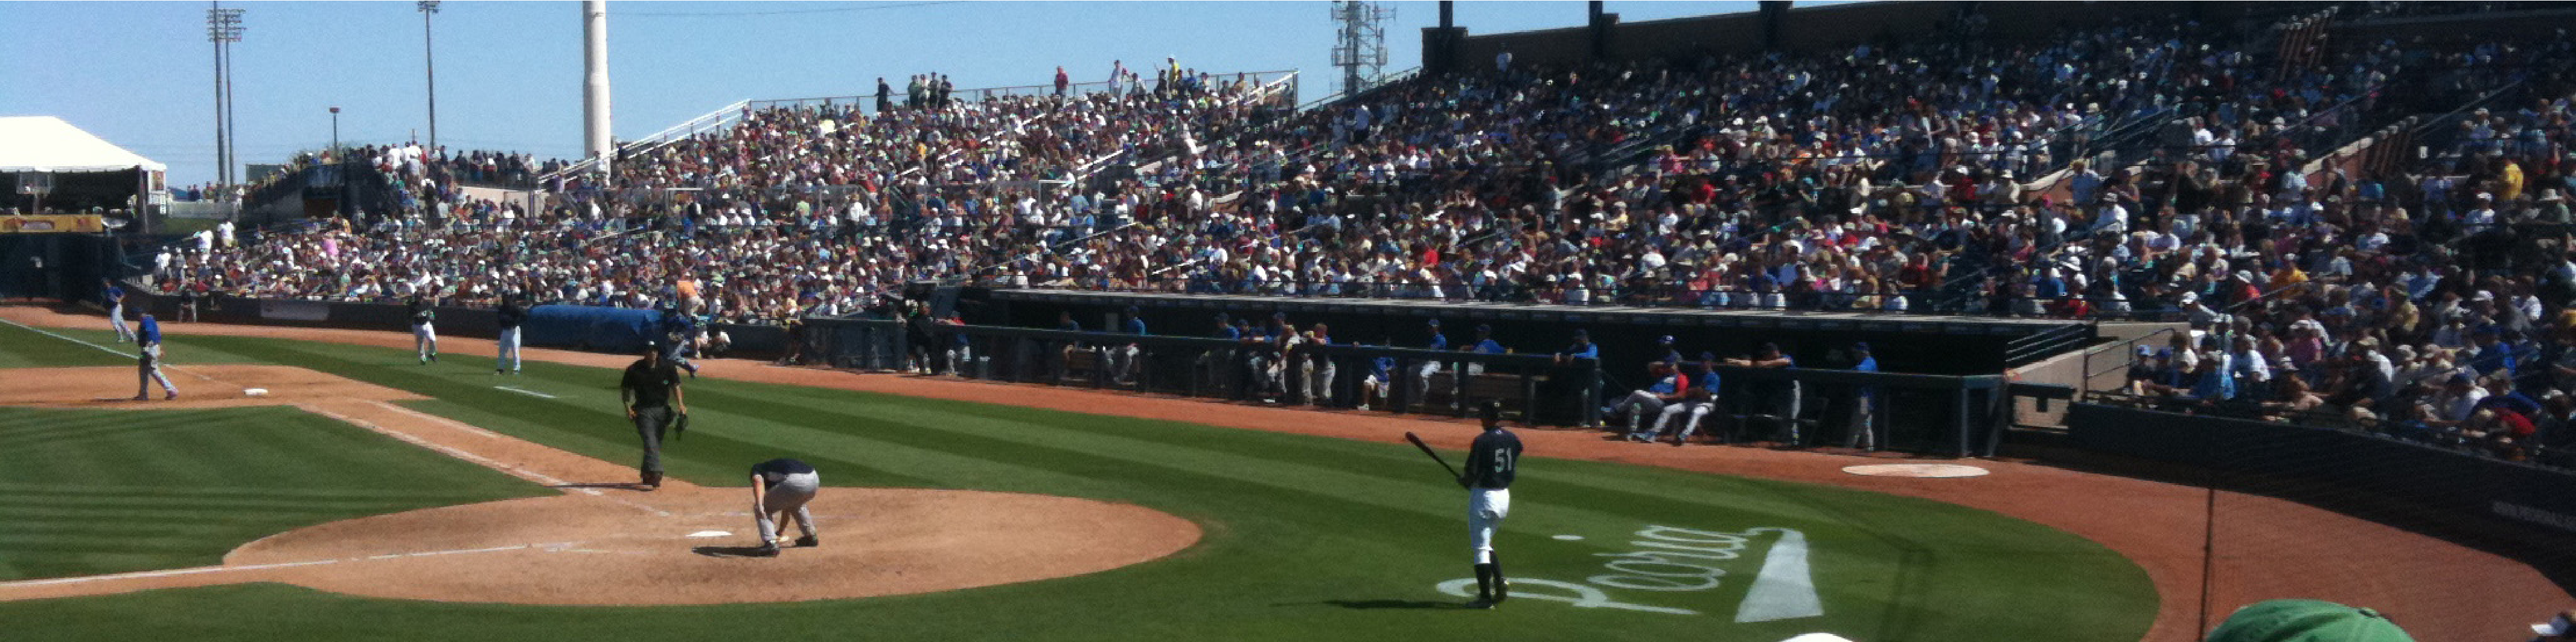
\includegraphics[width=\textwidth]{sampleteaser}
%  \caption{Seattle Mariners at Spring Training, 2010.}
%  \Description{Enjoying the baseball game from the third-base 
% seats. Ichiro Suzuki preparing to bat.} 
%  \label{fig:teaser} 
%\end{teaserfigure} 

%% 
%% This command processes the author and affiliation and title 
%% information and builds the first part of the formatted document. 

\maketitle 

\section{Introduction}
\label{sec:intro} 
Improving user engagement and preventing user churn have become an important focus for many internet companies as the market matures and the cost of acquiring new users rises. In addition to the natural friction, experiencing poor service is one of the main driving factors behind user churn. In different industries, companies provide different services, examples include  ride-sharing (Uber, Lyft), accommodation (Airbnb), and e-commerce (Amazon, Ebay).

As suggested in previous research [1] from Uber, providing a user with a promotion without explicit apology after an unsatisfactory trip experience will have a positive treatment effect on future billings. This is consistent with the finding in [2] where researchers conducted a similar experiment on Via (a ride-sharing company in NYC). However previous research and common practice relies on non-causal churn prediction or heuristics based on frustrating experiences for promo decisions instead of directly optimizing for users' treatment effects under a cost constraint. 

The goal of our work is to provide a framework to directly optimize for the overall effectiveness of treatments. This framework has the combined effect of minimizing cost and creating uplift in user engagement. Compared to existing work, novel contributions of this paper are: 

\begin{itemize}

\item \textbf{Heterogeneous Treatment Effect based Business Decisions} - A common approach for user promo decisions relies on regular predictions, redemption or heuristics which are tied to specific scenario and require rich background context. In this paper we propose a general framework that directly optimizes the heterogeneous treatment effect and could be applied to various business use cases with minimum change. This approach can be evaluated effectively and give guidance to decisions. 

\item \textbf{Optimization for Aggregated Treatment Efficiency} - Most research studies focus on treatment effect of one single outcome. However, in real-world applications it’s necessary to consider treatment effect on the cost, i.e. the efficiency ratio of  $\delta$cost/$\delta$value when making the resource allocation decision. Common approach also only considers point estimates but our objective is to maximize effectiveness from aggregated treatment effect. Our proposed framework will solve these two challenges together.

\item \textbf{Deep Learning with Causal Effectiveness Objective} - We derive from first principles the causal inference objective function to optimizes for treatment effectiveness. We develop methodologies in deep learning to dynamically focus on important users and incorporate resource constraints, such as limited budget, into the optimization algorithm. The objective is generalized into a casal learning loss layer that can be utilized in deep learning models. We demonstrate superior algorithmic flexibility of this modeling framework evidenced by experimentation.

\item \textbf{Recurrent Sequential Model for Treatment Cadence} - Cadence or sequences of treatments affect user behavior in sophisticated ways. These treatments and user state variations over time form a novel problem space. We formulate a sequential causal learning algorithm to learn combined effect of actions across many treatment periods. This is a all-purpose model that can be used to model both short-term and long-term treatment effects.
\end{itemize} 

The structure of this paper is as follows: in Section~\ref{sec:related_work}, we will cover related work in optimization of treatment effect. In Section~\ref{sec:algorithms}, we make the problem statement and introduce effectiveness measures and our modeling approaches for treatment effect optimization. In Section~\ref{sec:empirical_results}, we will cover experimentation, results, comparisons across models and real-world performance from the product we launched. Finally we briefly cover future research steps. 
\vspace{-0.2cm}
\section{Background} 
\label{sec:related_work} 
Methods optimizing for user retention have been widely studied. Two recent studies by Halperin et al. [1] and Cohen et al. [2]  look into the effect of apology treatments when the user's trust is compromised. Andrews et al. [19] studied factors that affect coupon redemption. Hanna et al. [20] and Manzoor and Akoglu [21] investigated factors that influence redemption of time limited incentives. These studies focus on redemption or exploratory average treatment effect and do not explore the optimization of user selection. 

The above methods attempt to solve the business problem, and do not yet apply a causal learning approach. ~\cite{rubin1974estimating} first brought forward a framework for studying treatment effects. User instances are treated with an action, and when the outcome is observed it is used in model fitting. One significant area is application of statistical methods such as~\cite{kunzel2017meta} that decomposes the learning algorithm into composite models with \emph{meta-learners}. The study of \emph{meta-learners} have developed to a variety of models. Another area is application of decision trees and random forests~\cite{chen2016xgboost}~\cite{ye2018rapidscorer}, for instance, uplift tree\cite{rzepakowski2012decision}, causal tree and random forests~\cite{wager2017estimation} , boosting~\cite{powers2017some} are powerful components to build causal inference models. Recently, another widely-adopted framework for learning heterogeneous treatment effect is the work of quasi-oracle estimation by~\cite{nie2017quasi}, which is proven to be effective when estimating the treatment effect in a single outcome. These methods consider both the \emph{Conditional Treatment Effect (CTE)} and the \emph{Average Treatment Effect (ATE)}. The \emph{CTE} is the treatment effect predicted by the model per sample conditional on its features while \emph{ATE} is the overall treatment effect. However, these algorithms are designed to estimate \emph{ATE} and \emph{CTE} for single outcome but could not deal with multiple outcomes and benefit-cost trade off. In this work we propose a set of algorithms which not only able to predict effect of treatment, but also combine multiple outcomes into real-world effectiveness measures that can be optimized directly using deep learning. 

\vspace{-0.2cm}
\subsection{Estimation of Treatment Effect} 
We start with the estimation of treatment effects with the potential outcomes framework (Neyman, 1923~\cite{neyman23thesis}; Rubin, 1974~\cite{rubin1974estimating}) consistent with prior work~\cite{nie2017quasi}. In the user retention case, users are $n$ independent and identically distributed examples indexed by $i$, where $\mathbf{X}^{(i)}$ denotes per-sample features for user $i$ while $\mathbf{X}$ is the entire dataset, $Y_1^{(i)}$ is the observed outcome if treated, and $Y_0^{(i)}$ is observed outcome if not treated. $T^{(i)}$ is the treatment assignment and is binary for a particular treatment type, i.e. $T^{(i)} \in \{0, 1\}$. 

We assume the treatment assignment is unconfounded, i.e., the outcome pair is independent of treatment label given the user features, or treatment assignment is as good as random once we control for the features  (Rosenbaum and Rubin, 1983~\cite{Rosenbaum83propensity}): $\{Y_0, Y_1\} \perp T_i|\mathbf{X}_i$. This is the assumption we make on all causal models we explore in the paper. The treatment propensity, probability of a user receiving treatment as $e(\mathbf{x}^{(i)}) = P (T = 1  | \mathbf{X}^{(i)} = \mathbf{x}^{(i)})$. 

With experiments, outcomes are observed given the treatment assignments. With each user we would have only observed one outcome per treatment. This historical data can be used to fit a model. For treatment effect estimation, we seek to estimate the treatment effect function given that we observe user features $X$: 
\vspace{-0.2cm}
\begin{align} 
\tau^*(\mathbf{x}) = E(Y_1 - Y_0 | \mathbf{X} = \mathbf{x})
\end{align} 
\vspace{-0.8cm}

\subsection{Quasi-oracle Estimation (R-learner)} 
Closely related to our work, we briefly review of the quasi-oracle estimation algorithm~\cite{nie2017quasi} for heterogeneous treatment effects, also known as \emph{`R-learner'}. The quasi-oracle estimation algorithm is a two-step algorithm for observational studies of treatment effects. The marginal effects and treatment propensities are first evaluated to form an objective function that isolates the causal component of the signal. Then the algorithm optimizes for the up-lift or causal component using regression. 

Concretely, the conditional mean of outcomes giving user features are $\mu^{*}_T(\mathbf{x}) = E(Y_T | \mathbf{X} = \mathbf{x})$, thus expected value of outcome from the model is $E(Y_T^{(i)} | \mathbf{X}^{(i)}) = E(Y_0^{(i)} | \mathbf{X}^{(i)}) + T^{(i)} E(Y_1^{(i)} - Y_0^{(i)} | \mathbf{X}^{(i)}) = \mu^*_0(\mathbf{X}^{(i)}) + T^{(i)}\tau^*(\mathbf{X}^{(i)})$. The expected value of the error $\epsilon$ across data and expected value of Y is zero given unconfoundedness assumption: \vspace{-0.2cm}
\begin{align} 
E(\epsilon(T^{(i)}) | \mathbf{X}^{(i)}, T^{(i)}) = 0
\end{align} 
\vspace{-0.1cm}
Replacing $E(Y_T^{(i)})$ in the error, and substitute the conditional mean outcome: $\epsilon(T^{(i)}) = Y_T^{(i)} - E(Y_T^{(i)}) = Y_T^{(i)} - (\mu^*_0(\mathbf{X}^{(i)}) + T^{(i)}\tau^*(\mathbf{X}^{(i)}))$; $m^*(\mathbf{x}^{(i)}) = E(Y^{(i)} | \mathbf{X}^{(i)} = \mathbf{x}^{(i)})$, we arrive at the decomposition: 
\vspace{-0.2cm}
\begin{align}
\label{eq:quasi_oracle_balance}
Y^{(i)} - m^*(\mathbf{X}^{(i)}) = (T^{(i)} - e^*(\mathbf{X}^{(i)})\tau^*(\mathbf{X}^{(i)}) + \epsilon
\end{align}
\vspace{-0.1cm} 
An equation that balances difference between outcome with a `mean' model with the conditional average treatment effect function. In a simple formulation of the quasi-oracle estimation algorithm a regression is used to fit the $m^*$ and $e^*$ models as the first step. The prediction result of the regression is then used to determine the regression target of $\tau^*$ model, which is then fitted also as a regression. After the learning, $\tau^*$ function can be used to estimate the treatment effect given user with feature $\mathbf{X}^{(i)}$. 

%Here we consider R-learner and Causal Forest as the treatment effect estimator. R-learner is a synthetic control fashion two-step algorithm that estimates the marginal effect and then isolates the causal component. Causal Forest is a matching fashion tree-based ensemble algorithm that directly estimates the treatment effect under each tree leaf. Generally we can train above models and have cardinal predictions $\hat{\tau}(x_i)$ for value (retention) and cost. 

%Data science efforts have also surveyed effective models and explore multiple treatments using A/B testing~\cite{}. 
%Due to significant interest to develop flexible and effective algorithms, the work is sub-divided into area

%These advances include methods based on Lasso [22], meta learners [9], recursive partitioning [5], neural networks [7], and most recently quasi-oracle estimation [3]. A recent survey by Dorie et al. [8] used  simulations and empirical datasets to show that these estimators can achieve good heterogeneous treatment effect estimation. However, they didn’t consider the special case of a constraint optimization problem where both cost and value are treatment effects. 

%Optimization. Our problem could be formed as a Knapsack problem [17]. Due to the large number of items and the small scale of the value and cost for each item, greedy approximation can achieve decent results [18]. That said, this work can also use some other optimization algorithm such as SGD [12] and Adam optimizer [13]. These two algorithms are implemented in TensorFlow [15] and provide the foundation for training of our methodology.

\vspace{-0.3cm}
\section{Algorithms} 
\label{sec:algorithms} 
\subsection{Problem Statement: Balanced Effectiveness} 
The quasi-oracle estimation algorithm, among other meta-learner algorithms~\cite{kunzel2017meta}, is efficient for estimating conditional treatment effects. However, treatment commonly leads to changes in multiple outcomes. For instance, a retention reward could lead to the user coming back to the platform and making more transactions, it also lead to a variable increase in cost including the retention cost, offset by the user's positive contributions. Sometimes these different outcomes cannot be converted to the same unit, for example if we want to boost trip growth by increasing the dollar spend on promotion, trip number and dollar spend cannot be converted to a single value. So the eventual goal is to maximize gains and with a cost constraint. Many problems in causal learning and reinforcement learning domain trades off the cost of action taking, with the reward obtained by those  actions~\cite{sutton18reinforcement}~\cite{silver16master}~\cite{kool2017cost}. Thus cost effectiveness is a key theme in data science applications of causal inference. In this paper, we propose causal inference paradigm to maximize cost effectiveness of heterogeneous treatments. 

Concretely, we refresh the problem statement. Instead of estimating the treatment effect function $\tau^*(\mathbf{x}) = E(Y_1 - Y_0 | \mathbf{X} = \mathbf{x})$, we propose to solve the problem illustrated below to maximize the gain outcome given a cost constraint. 
\vspace{-0.3cm}
\begin{align} 
\label{eq:pstatement_constrained} 
\begin{split}
  \text{maximize} \quad &\sum_{i=1}^n\tau^{*r}(\mathbf{x}^{(i)})z_i \\ 
  \text{subject to} \quad &\sum_{i=1}^n\tau^{*c}(\mathbf{x}^{(i)})z_i \leq B \\
	&z_i \in\{0, 1\} 
\end{split}
\end{align} 
The variables $z_i$ represent whether we offer a reward to the user during a campaign and $B$ is the cost constraint. We represent retention treatment effects as $\tau^{*r}(\mathbf{x}^{(i)}) = E(Y_1^r - Y_0^r | \mathbf{X}^{(i)} = \mathbf{x}^{(i)})$ and cost as $\tau^{*c}(\mathbf{x}^{(i)}) = E(Y_1^c - Y_0^c | \mathbf{X}^{(i)} = \mathbf{x}^{(i)})$. It is important to note these treatment effect values are part of the optimization objective and are implicitly modeled as intermediate quantities. They are not strictly regression functions, and we holistically solve the stated problem. 
\vspace{-0.2cm}
\subsection{Duality R-learner} 
We describe the duality method with Lagrangian multipliers to solve the constrained optimization problem for maximizing gain (minimizing negative gain) subject to a budget ($B>0$) constraint, and relaxing the previous $z_i\in\{0, 1\}$ variables to continuous: 
\vspace{-0.25cm}
\begin{align} 
\label{eq:constrained_problem} 
\begin{split}
  \text{minimize} \quad -&\sum_{i=1}^n\tau^{*r}(\mathbf{x}^{(i)})z_i \\ 
  \text{subject to} \quad &\sum_{i=1}^n\tau^{*c}(\mathbf{x}^{(i)})z_i \leq B \\
	&\ 0\leq z_i \leq 1 
\end{split}
\end{align} 
\vspace{-0.1cm}
First, we assume the CATE functions are fixed, so we solve Problem~\ref{eq:pstatement_constrained} assuming $\tau^{*r}(\mathbf{x}^{(i)})$ and $\tau^{*c}(\mathbf{x}^{(i)})$ are given. Applying one Lagrangian multiplier, the Lagrangian for Problem~\ref{eq:pstatement_constrained}: 
\vspace{-0.2cm}
\begin{equation} 
  \label{eq:lagrangian} 
  L(\mathbf{z}, \lambda)=-\sum_{i=1}^n\tau^{*r}(\mathbf{x}^{(i)})z_i + \lambda (\sum_{i=1}^n\tau^{*c}(\mathbf{x}^{(i)})z_i - B) \\ 
\end{equation} 
\vspace{-0.1cm}
The optimization in Problem~\ref{eq:pstatement_constrained} can then be rewritten in its Dual form to maximize the Lagrangian dual function $g = \inf_{\mathbf{z}\in\emph{D}}L(\mathbf{z}, \lambda)$: 
\vspace{-0.1cm}
\begin{align} 
\label{eq:duality_problem} 
\begin{split}
  \max\limits_{\lambda} \inf_{\mathbf{z} \in \emph{D}} L(\mathbf{z}, \lambda) \quad
  \text{subject to} \ 0\leq z_i \leq 1, \lambda \geq 0 \\
\end{split}
\end{align} 
We need to address the caveats for solving the problem with duality, and determine whether the dual problem has the same minimum with original problem.
\begin{itemize} 
\item If $p(\mathbf{z}, \lambda) = -\sum_{i=1}^n\tau^{*r}(\mathbf{x}^{(i)})z_i$, we know, for the optimal values of the two problems, $p^* \leq g^*$ holds from convex optimization. Equality $p^* = g^*$ holds if $p$, $g$ are convex, and the \emph{Slater constraint qualification} holds, which requires the problem to be strictly feasible. 
\item For any values of $B > 0$, if we consider very small values of some $z_i$, the strict inequality $\sum_{i=1}^n\tau^{*c}(\mathbf{x}^{(i)})z_i < B$ can always hold. Further, $B$ is usually large for a promotion campaign. Thus Slater qualifications hold. 
\end{itemize} 

From the analysis above, Problem~\ref{eq:pstatement_constrained} and its dual problem~\ref{eq:duality_problem} are equivalent, and we can solve Problem~\ref{eq:duality_problem} by iteratively optimizing with respect to $\mathbf{z}, \lambda$.  

\textbf{Optimize $\mathbf{z_i}$:} Keeping $\lambda, \mathbf{\tau}$ fixed, as $\lambda$ and $\ B$ are constants, Problem~\ref{eq:duality_problem} becomes: 
\vspace{-0.3cm}
\begin{equation} 
\begin{split}
  \label{eq:lagrangian_reduced}
  \text{maximize}\quad \sum_{i=1}^nz_i s_i \\
  \text{subject to} \quad 0\leq z_i \leq 1
\end{split}
\end{equation} 
Where we define the \emph{effectiveness score} $s_i = \tau^{*r}(\mathbf{x}^{(i)})-\lambda\tau^{*c}(\mathbf{x}^{(i)})$. This optimization problem has a straightforward solution: assign the multiplier $z_i = 1$ when the ranking score $s_i \geq 0$ and assign $z_i = 0$ when ranking score $s_i < 0$. 

\textbf{Optimize $\lambda$:} Take the derivative of $L$ with regards to $\lambda$, $\frac{\partial g}{\partial \lambda}=B-\sum_{i=1}^n\tau^{*c}(\mathbf{x}^{(i)})z_i$. We can update $\lambda$ by Eq. (\ref{eq:update_lambda}) where $\alpha$ is the learning rate. \vspace{-0.1cm}
\begin{equation}
  \label{eq:update_lambda}
  \lambda\rightarrow \lambda + \alpha(B-\sum_{i=1}^n\tau^{*c}(\mathbf{x}^{(i)}))
\end{equation}
Based on the two steps above, we can iteratively solve for both $z_i$ and $\lambda$ \cite{bertsekas1999nonlinear} .

In the next part, we solve for the $\tau^*$ functions, then finally connect components together to form the eventual algorithm. We can leverage quasi-oracle estimation of the CATE function $\tau$~\cite{nie2017quasi}. Concretely, the $m^*$ function, and optionally $e^*$ function, are fitted with L2 regularized linear regression, then $\tau^*$ functions are fitted with Eq.~\ref{eq:quasi_oracle_balance}. The problems are convex and have deterministic solutions. 

In our \emph{Duality R-learner} algorithm, we take an approach to combine the two $\tau^*$ functions into one model. Instead of learning $\tau^{*r}$ and $\tau^{*c}$ respectively, we fit a single \emph{scoring model} $s_i=\tau^{*E}(\mathbf{x}^{(i)})$ in Eq.~\ref{eq:lagrangian_score}. Note the Duality solution suggests we should include any sample with $\hat\tau^{*E}(x_i)>0$. Larger this value, more contribution the sample will have and thus a higher ranking it should get. 
\begin{equation} 
  \label{eq:lagrangian_score} 
  s_i=\tau^{*E}(\mathbf{x}^{(i)})=\tau^{*r}(\mathbf{x}^{(i)})-\lambda\tau^{*c}(\mathbf{x}^{(i)}) 
\end{equation} 
This form is linear, so we can use $Y^E=Y^r-\lambda Y^c$ instead of the the original $Y$ (single outcome for value and cost respectively) in the estimators above. Specifically, Eq. (\ref{eq:lagrangian_linearity}). 
\begin{align} 
  \label{eq:lagrangian_linearity} 
  \tau^{*r}(\mathbf{x}) - \lambda \tau^{*c}(\mathbf{x}) &= E((Y^r_1 - \lambda Y^c_1 - (Y^r_0  - \lambda Y^c_0)| \mathbf{X} = \mathbf{x}) \\&= E(Y^E_1 - Y^E_0 | \mathbf{X} = \mathbf{x}) 
\end{align} 
Then we train a regression model through the quasi-oracle estimation method, with this $Y^E$ and the output becomes $\tau^{*E}$ which could be used directly. This has two benefits: first, we optimize a joint model across $Y^r$ and $Y^c$ for the parameters to be able to find correlations jointly; second, for production and online service, we will arrive at one single model to perform prediction. 

%The iterative process to solve $\lambda$ could be slow as the value function $g$ here is piece-wise linear w.r.t $\lambda$. We take the approach to treat $\lambda$ as a hyper-parameter and determine its value through hyper-parameter optimization. 

We iteratively solve the Duality R-learner algorithm. This duality method lightens the production burden of having multiple models, and the algorithm can jointly improve cost and benefit by directly solving the constrained optimization problem for balanced effectiveness. %eliminates any noise introduced by divided predicted values of $\frac{\tau^{*c}}{\tau^{*r}}$. %Figure \ref{fig:cc_lagrangian_vs_ratio} shows the out-of-sample test cost curve comparison between Lagrangian and Causal Ratio using Causal Forest. We used data collected from our promotion experiment (details in \ref{experiment design and ata}) and optimize hyper-parameters with forward validation(details in \ref{offline test setup}). We can see that the Lagrangian model dominates the Causal Ratio model. 
\vspace{-0.2cm}
\subsection{Direct Ranking Model} 
The approach described in the previous section contains two separate steps, treatment effect prediction and constraint optimization. The ultimate business objective is to identify a \emph{portfolio of users} that we can achieve highest incremental user retention with a cost budget, which does not rely on the perfect individual prediction (point estimate) of treatment effect, but rather, achieves the overall market-wide effectiveness. This is similar to the search ranking algorithm to optimize for a holistic ranking objective vs Click Through Rate (CTR) point  estimate~\cite{huang2013learning}~\cite{shen2014a}. We aim to achieve better performance by combining these two steps together, and this is the algorithm we propose: Direct Ranking Model (DRM). 

This model tries to solve an unconstrained optimization problem where we minimize the cost per unit of gain: 
\begin{align} 
\label{eq:pstatement_unconstrained_opt} 
\text{minimize} \quad \frac{\bar{\tau}^{*c}(\mathbf{x})}{\bar{\tau}^{*r}(\mathbf{x})} 
\end{align} 

The overlined treatment effect quantities for retention gains $\overline{\tau}^{*r}(\mathbf{x}) = E(Y_1^r - Y_0^r | \mathbf{X} = \{\mathbf{x}^{(i)}\})$ and cost $\overline{\tau}^{*c}(\mathbf{x}) = E(Y_1^c - Y_0^c | \mathbf{X} = \{\mathbf{x}^{(i)}\})$ are expectations across selected user portfolio. We can directly optimize for this market-wide effectiveness. The cost per unit gain objective allows us to take all users and outcomes into consideration. The unconstrained optimization allows us to utilize deep learning to build flexible models and efficiently train with large-scale data. 

\textbf{Derivation with Causal Inference.} We derive the objective function of the Direct Ranking Model stated in Problem~\ref{eq:pstatement_unconstrained_opt}. Without loss generality we include per sample treatment propensity from causal statistics~\cite{lunceford04stratification} and derive $\bar{\tau}$ without superscript as it could extend to both $\bar{\tau}^{*r}$ and $\bar{\tau}^{*c}$. Start from the fundamental definition of treatment effect: 
\begin{align*}   
\bar{\tau}^{*} &= E(Y_1 - Y_0) = E(Y_1) - E(Y_0) 
\end{align*}
From~\cite{lunceford04stratification}, the expected value of outcome given treatment or non-treatment of any user can be written as following equations. This takes treatment label and propensities into account: 
%\footnote{$E(Y_1) = E(\frac{Y_1}{e(X)} e(X)) = E(\frac{Y_1}{e(X)}E(T | X)) = E(\frac{Y_1}{e(X)}E(T | X, Y_1)) = E(E(\frac{Y_1T}{e(X)} | X, Y_1)) = E(\frac{Y_1T}{e(X)})$}
\begin{align} 
E(Y_1) = E(\frac{Y_1T}{e(\mathbf{x})}),  \quad E(Y_0) = E(\frac{Y_0 (1-T)}{1-e(\mathbf{x})})
\end{align} 
$e(\mathbf{x})$ is a propensity function which indicates probability of treatment, or $E(T=1|\mathbf{X} = \mathbf{x})$. This quantity is estimated per user given their features, thus is a learnable propensity function fitted with the user feature and treatment labels. Detailed proof of the above equation is given for $Y_1$ case: $E(Y_1) = E(\frac{Y_1}{e(\mathbf{x})} e(\mathbf{x})) = E(\frac{Y_1}{e(\mathbf{x})}E(T | \mathbf{X}=\mathbf{x})) = E(\frac{Y_1}{e(\mathbf{x})}E(T | \mathbf{X}=\mathbf{x}, Y_1)) = E(E(\frac{Y_1T}{e(\mathbf{x})} | X, Y_1)) = E(\frac{Y_1T}{e(\mathbf{x})})$\footnote{Third step follows from unconfoundedness assumption~\cite{lunceford04stratification}~\cite{nie2017quasi}.} 

We then go ahead to substitute into the treatment effect definition: 
%As stated above, users are evaluated with an \emph{effectiveness measure}, $p_i$. This measure is across all users, and semantics of a larger $p_i$ is the user is more cost-efficient to send treatment, thus more likely to be selected into our portfolio. 
\vspace{-0.1cm}
\begin{align} 
\label{eq:drm_propensity_1} 
\begin{split} 
\bar{\tau^{*}} &= E(Y_1 - Y_0) = E(Y_1) - E(Y_0) \\
&= E(\frac{Y_1T}{e(\mathbf{x})})  - E(\frac{Y_0 (1-T)}{1-e(\mathbf{x})}) \\ 
&= E(E(\frac{Y_1T}{e(\mathbf{x})}|T)) - E(E(\frac{Y_0(1-T)}{1-e(\mathbf{x})}|T)) \\ 
\end{split} 
\end{align} 
The last step follows from law of total expectation. We can then expand the equation by definition of expectation: 
\vspace{-0.1cm}
\begin{align} 
\label{eq:drm_propensity_2} 
\begin{split} 
\vspace{-0.1cm}
\bar{\tau}^{*} &= P(T = 1) E(\frac{Y_1T}{e(\mathbf{x})}|T = 1) + \cancel{P(T = 0) E(\frac{Y_1T}{e(\mathbf{x})}| T = 0)} \\
&\quad - \cancel{P(T = 1) E(\frac{Y_0 (1-T)}{1-e(\mathbf{x})}|T = 1)} - P(T = 0) E(\frac{Y_0 (1-T)}{1-e(\mathbf{x})} | T = 0) 
\end{split} 
\end{align} 
For each user, we use $p_i$ as a relaxation of the binary decision variable $z_i$ in the previous problem, the effectiveness weighting to select user $i$. The higher the $p_i$, the higher likelihood of selecting the sample, and we constrain $\sum p_{i, T_i = 0} = 1$, $\sum p_{i, T_i=1} = 1$, i.e. the effectiveness measures for users in the treatment cohort, and control cohort sums to $1$ respectively. This normalization gives the effective measure a probabilistic interpretation. We define $\hat{e}$ to be the overall propensity, or probability of treatment, estimated by mean of the binary treatment labels across users. For each user, the $e(\mathbf{x})$ term is estimated from a pretrained propensity function. Then, we expand the expectation terms $E(\frac{Y_1T}{e(\mathbf{x})}|T = 1)$, $E(\frac{Y_0 (1-T)}{1-e(\mathbf{x})} | T = 0)$ using the normalized effectiveness weighting, potential outcomes $Y^{(i)}_1$, $Y^{(i)}_0$ and observed outcome labels $Y^{(i)}$: 
\vspace{-0.2cm}
\begin{align} 
\label{eq:drm_propensity_3} 
\begin{split} 
\bar{\tau}^{*} &= \hat{e} \sum_{T_i =1} \frac{Y^{(i)}_1 p_{i}}{e(\mathbf{x}^{(i)})} - (1-\hat{e}) \sum_{T_i = 0} \frac{Y^{(i)}_0 p_i}{1-e(\mathbf{x}^{(i)})} \\ 
& = \hat{e} \sum_{i=1}^n \frac{1}{e(\mathbf{x}^{(i)})} Y^{(i)}_1 p_{i} \mathbb{I}_{T_i=1} - (1-\hat{e}) \sum_{i = 0}^n \frac{1}{1-e(\mathbf{x}^{(i)})} Y^{(i)}_0 p_i \mathbb{I}_{T_i=0} \\ 
& = \hat{e} \sum_{i=1}^n \frac{1}{e(\mathbf{x}^{(i)})} Y^{(i)} p_{i} \mathbb{I}_{T_i=1} - (1-\hat{e}) \sum_{i = 0}^n \frac{1}{1-e(\mathbf{x}^{(i)})} Y^{(i)} p_i \mathbb{I}_{T_i=0}
\end{split} 
\end{align} 
Eq.~\ref{eq:drm_propensity_3} is a generalized form of the $\bar{\tau}^{*}$ including part of the objective function with propensity weighting. When $\hat{e} = e(\mathbf{x}^{(i)})$ is constant in a fully randomized experiment, the term becomes: %, and the last line uses a sampling approximation, where $p_u(X)$ is the discrete probability density given by user sampler, normalized with respect to treatment and control cohorts, respectively. This sampler could be used as a ranker at inference time to determine the users to apply treatment. 
\vspace{-0.1cm}
\begin{align} 
\label{eq:drm_propensity_4} 
\begin{split} 
  \bar\tau^{*}=\sum_{i=1}^n Y^{(i)}p_i(\mathbb{I}_{T_i=1} - \mathbb{I}_{T_i=0})
\end{split} 
\end{align} 
\vspace{-0.1cm}
\textbf{Model and Effectiveness Objective.} Using the above derivations, we can then construct our model and the loss function as follow. In Eq. (\ref{eq:drm_1}) $f$ is the function the model will learn with tunable parameters. This function outputs an effectiveness score, indicating how efficient the sample is based on its features $\mathbf{x^{(i)}}$. $f$ can be in any differentiable form such as linear or a neural network structure. 
\begin{equation}
  \label{eq:drm_1} 
  S_i = f(\mathbf{x}^{(i)}) 
\end{equation} 
We use a standard hyperbolic tangent as non-linear activation for the neural network($\tanh$). 
\begin{equation} 
  \label{eq:drm_2}
  s_i = \tanh(S_i)
\end{equation}
We then normalize the effectiveness scores using the softmax function to arrive at $p_i$ for each user (Eq. (\ref{eq:drm_3_1})). $p_i$ sum to 1 in each cohort respectively, for $T_i=1$ and $T_i=0$. 
\begin{equation}
  \label{eq:drm_3_1}
  p_i = \frac{e^{s_i}}{\sum_{j=1}^n\mathbb{I}_{T_j=T_i}e^{s_j}}
\end{equation}
Here $\mathbb{I}_{T_j=T_i}$ is the indicator function for sample $j$ whether it's in the same group (treatment or control) as sample $i$. 
%It could be expanded as Eq. (\ref{eq:drm_3_2}) and Eq. (\ref{eq:drm_3_3}).
%\begin{equation}
%  \label{eq:drm_3_2}
%  p_{i, T_i=1} = \frac{e^{s_i}}{\sum_{\{j:T_j=1\}}e^{s_j}}
%\end{equation}
%\begin{equation}
%  \label{eq:drm_3_3}
%  p_{i, T_i=0} = \frac{e^{s_i}}{\sum_{\{j:T_j=0\}}e^{s_j}}
%\end{equation} 
Based on this, we can calculate the expected treatment effect of our user portfolio using the derived Eq.~\ref{eq:drm_propensity_4}. We can write effectiveness weighted sample treatment effect for retention and cost with (Eq. (\ref{eq:drm_4_1}), Eq. (\ref{eq:drm_4_2})).
\vspace{-0.1cm}
\begin{equation}
  \label{eq:drm_4_1}
  \bar\tau^{*r}=\sum_{i=1}^nY^{r(i)}p_i(\mathbb{I}_{T_i=1} - \mathbb{I}_{T_i=0})
\end{equation}
\vspace{-0.1cm}
\begin{equation}
  \label{eq:drm_4_2}
  \bar\tau^{*c}=\sum_{i=1}^nY^{c(i)}p_i(\mathbb{I}_{T_i=1} - \mathbb{I}_{T_i=0})
\end{equation}
\vspace{-0.1cm}
Finally, we have our loss function in Eq. (\ref{eq:drm_5}), which is the ratio of treatment effects as the holistic efficiency measure plus a regularization term.
\vspace{-0.1cm}
\begin{equation}
  \label{eq:drm_5}
  \hat{f}(\cdot ) = argmin_{f}\left \{ \frac{\bar{\tau^c}}{\bar{\tau^r}}+\Lambda_n(f(\cdot ))  \right \}
\end{equation}
\vspace{-0.1cm}
Since all the operations above are differentiable, we can use any off-the-shelf optimization method to minimize the loss function and learn the function $f$. Because the direct optimization is well suited for deep learning, we incorporated this method with the deep learning architectures and frameworks, and implemented our approach using TensorFlow \cite{abadi2016tensorflow} and used Adam optimizer \cite{kingma2014adam}. The definition of $f$ function is flexible for instance, multi-layer neural networks, convolutional and recurrent networks. 

%In our algorithm, one caveat is it is possible to output high score to several samples which generate great treatment effect and ignore others. In addition to the general regularization term on weights in loss function, we use equation (2) to prevent this degenerate mode. Since $\tanh$ will saturate gradients for large absolute value. This prevents the algorithm from assigning ever larger scores to a smaller sample and enables the model to generalize better to the data. 

%\textbf{Proof with Causal Inference.} We derive the objective function in Eq.~\ref{eq:drm_4_1}, Eq.~\ref{eq:drm_4_2}, and Eq.~\ref{eq:drm_5} of the Direct Ranking Model with generality of including treatment propensity from causal statistics~\cite{lunceford04stratification}. The expected value of outcome given treatment or non-treatment of any user is: 

%\footnote{$E(Y_1) = E(\frac{Y_1}{e(X)} e(X)) = E(\frac{Y_1}{e(X)}E(T | X)) = E(\frac{Y_1}{e(X)}E(T | X, Y_1)) = E(E(\frac{Y_1T}{e(X)} | X, Y_1)) = E(\frac{Y_1T}{e(X)})$}
%\begin{align} 
%E(Y_1) = E(\frac{Y_1T}{e(\mathbf{x})}),  \quad E(Y_0) = E(\frac{Y_0 (1-T)}{1-e(\mathbf{x})})
%\end{align} 
%$e(\mathbf{x})$ is a propensity function which indicates probability of treatment, or $E(T=1|\mathbf{X} = \mathbf{x})$.  Detailed proof is given for $Y_1$ case as: $E(Y_1) = E(\frac{Y_1}{e(\mathbf{x})} e(\mathbf{x})) = E(\frac{Y_1}{e(\mathbf{x})}E(T | \mathbf{X}=\mathbf{x})) = E(\frac{Y_1}{e(\mathbf{x})}E(T | \mathbf{X}=\mathbf{x}, Y_1)) = E(E(\frac{Y_1T}{e(\mathbf{x})} | X, Y_1)) = E(\frac{Y_1T}{e(\mathbf{x})})$\footnote{Third step follows from unconfoundedness assumption~\cite{lunceford04stratification}~\cite{nie2017quasi}.} 

%As stated above, users are evaluated with an \emph{effectiveness measure}, $p_i$. This measure is across all users, and semantics of a larger $p_i$ is the user is more cost-efficient to send treatment, thus more likely to be selected into our portfolio. 
%\begin{align} 
%\label{eq:drm_propensity} 
%\begin{split} 
%\tau^{*r} &= E(Y_1 - Y_0) = E(Y_1) - E(Y_0) \\
%&= E(\frac{Y_1T}{e(\mathbf{x})})  - E(\frac{Y_0 (1-T)}{1-e(\mathbf{x})}) = E_T(E(\frac{Y_1T}{e(\mathbf{x})}|T)) - %E_T(E(\frac{Y_0(1-T)}{1-e(\mathbf{x})}|T)) \\ 
%& = P(T = 1) E(\frac{Y_1T}{e(\mathbf{x})}|T = 1) + \cancelto{0}{P(T = 0) E(\frac{Y_1T}{e(\mathbf{x})}| T = 0)} \\
%&\quad - \cancelto{0}{P(T = 1) E(\frac{Y_0 (1-T)}{1-e(\mathbf{x})}|T = 1)} - P(T = 0) E(\frac{Y_0 (1-T)}{1-e(\mathbf{x})} | T = 0) \\
%& = \hat{e} \sum_{T_i =1} \frac{Y^{r(i)} p_{i}}{e(\mathbf{x}^{(i)})} - (1-\hat{e}) \sum_{T_i = 0} \frac{Y^{r(i)} p_i}{1-e(\mathbf{x}^{(i)})} \\ 
%& = \hat{e} \sum_{i=1}^n \frac{1}{e(\mathbf{x}^{(i)})} Y^{r(i)} p_{i} \mathbb{I}_{T_i=1} - (1-\hat{e}) \sum_{i = 0}^n \frac{1}{1-e(\mathbf{x}^{(i)})} Y^{r(i)} p_i \mathbb{I}_{T_i=0}
%\end{split} 
%\end{align} 

%Eq.~\ref{eq:drm_propensity} is a generalized form of Eq.~\ref{eq:drm_4_1} with propensity weighting. They are the same equation when $\hat{e} = e(\mathbf{x}^{(i)}) = 0.5$. $\hat{e}$ is the mean of the binary treatment labels across users.%, and the last line uses a sampling approximation, where $p_u(X)$ is the discrete probability density given by user sampler, normalized with respect to treatment and control cohorts, respectively. This sampler could be used as a ranker at inference time to determine the users to apply treatment. 

%Regularization for heterogeneous treatment effect. Any matching fashion method will face the overfitting issue that during training, the model can always try to match sample from treatment and control to exaggerate the heterogeneous effect. In Causal Forest, they used the honest split (use different data set for tree construction and leaf treatment effect estimation) to control this. In our algorithm, the caveat is it can put extremely high score to several samples which generate great treatment effect and ignore others. In addition to the general regularization term on weights in loss function, we also use equation (2) to control for this. Since $\tanh$ will be saturated for large absolute value, its gradient will diminish once  is relatively large. This prevents the algorithm from assigning ever larger scores to a smaller sample and forces it to find a general pattern which could be applied to a larger group. Empirically this performs well, and without the control of tanh, the algorithm will be easily overfitted. 

%With this normalized effectiveness, we could obtain the expected value of outcome $Y$ using training data observed from experiments. With these expected outcome values, we would incorporate the desired cost-efficiency measure When the probability density function is taken to be a differentiable function with respect to the user features, we can optimize the parameters of the  to obtain the most desired outcome which generalizes to test set given sufficiently large datasets. 

%In the above equation, $\hat{e}$ is the sample mean of the binary treatment labels across all users, and the last line uses a sampling approximation, where $p_u(X)$ is the discrete probability density given by user sampler, normalized with respect to treatment and control cohorts, respectively. This sampler could be used as a ranker at inference time to determine the users to apply treatment. 
\vspace{-0.2cm}
\subsection{Constrained Ranking Models} 

Constraints are inherent in retention and engagement products, such as a fixed cost budget or product limitations to send to only 30\% quantile of the users. Despite the previous model is able to directly optimize for market-wide effectiveness and utilize powerful deep learning models, the algorithm is disadvantaged with constraints and may not find the best solution. 

At the same time, there is difficulty to leverage deep learning models to solve hard-constrained optimization problems~\cite{marquez2017imposing}. To address these difficulties, we develop methods to turn hard constraints into soft constraints applicable to the deep learning methodology. Concretely, we enable this by developing two novel deep learning components: \emph{dynamic quantile pooling} and \emph{constraint annealing}.

\textbf{Dynamic Quantile Pooling} Many deep learning algorithms apply the critical step of \emph{pooling}. Pooling applies a mathematical operator such as $max$ or $mean$ to selectively retain values from the previous layer. These operations create useful sparsity in deep learning architectures which eases pressure on the sophisticated optimization process and increase invariance in the top layer representations~\cite{lecun1995convolutional}~\cite{zou2012deep}~\cite{jarrett2009best}~\cite{le2011learning}. In this section, we describe the new pooling method for selecting a quantile of effectiveness measures from the whole population using a sorting operator. This pooling component enables us to systematically select output satisfying constraints and dynamically construct efficiency objective focused on those selections. We propose this method with the deep learning architecture in our causal learning framework.

We assume either a quantile $q\%$ or a cost budget $B$ is given as a fixed hyper-parameter. For the former, we are constrained to offer treatment to top $q\%$ of the users, for the latter, we could not exceed the budget $B$. 

Leveraging methodologies developed in the previous section (Eq.~\ref{eq:drm_1}, Eq.~\ref{eq:drm_2}), at optimization iteration $(k)$, for user $(i)$ in the dataset, users' effectiveness score is calculated as below. Assume $s_i^{(k)}$ is the original score: 
\vspace{-0.2cm}
\begin{align*} 
	s_i^{(k)} = \tanh (f^{(k)}(\mathbf{x}^{(i)})) 
    %S_i^{(j)} = f^{(j)}(\mathbf{x}^{(i)})\quad s_i^{(j)} = \tanh (S_i^{(j)}) 
\end{align*} 
\vspace{-0.1cm}
The treatment decision depends on the value of $s_i^{(k)}$ and its mathematical relationship with our constraints. We abstract this treatment decision with a fall-off function $\sigma^*$ (chosen to be a \emph{sigmoid function}) and an input offset $d^{*(k)}$, shown in Eq.~\ref{eq:offset_fall_off}. It illustrates how this offset $d$ lead to a fall-off variable $v$ which discounts output scores. In this equation the $t^*$ variable is a hyperparameter called \emph{temperature} to control softness of the fall-off.
\vspace{-0.2cm}
\begin{align} 
\label{eq:offset_fall_off} 
	V_i^{(k)} = s_i^{(k)} - &d^{*(k)} \quad v_i^{(k)} = \sigma^* (V_i^{(k)}) = \frac{1}{1 + \exp(-t^*V_i^{(k)})}
\end{align} 
\vspace{-0.1cm} 
Here the offset $d_i$ is determined by both constraints and the population of scores $\mathbf{s}^{(k)}=\{s_i^{(k)}\}$ at iteration $(k)$. In this paper, we give two definitions of this offset transform: 

\textbf{\emph{Top Quantile Constraint}}: For optimization constrained to a fixed quantile $q\%$, we related the offset with a quantile function $\Gamma_Q(\mathbf{s^{(k)}}, q)$ where $q\%$ is the quantile percentage above which we decide to offer treatment:  
\vspace{-0.1cm}
\begin{align*} 
    d^{*(k)} = \Gamma_Q (\mathbf{s}^{(k)}, q) 
\end{align*} 
\vspace{-0.1cm}
The $\Gamma_Q$ function is implemented using a \emph{sorting operator} $\Psi$ and \emph{take $n$th} operator $\mu$, and $n = N\frac{q}{100}$ where N is total number of users in the population: 
\vspace{-0.1cm}
\begin{align*} 
	\Gamma_Q (\mathbf{s}^{(k)}, q) = \mu(\Psi(\mathbf{s}^{(k)}), n) 
\end{align*} 
\vspace{-0.1cm}
Semantically it means we first sort user effectiveness scores then take the q\% quantile value as offset $d^{(k)}$. 

\textbf{\emph{Fixed Cost Constraint}}: For optimization constrained to a fixed cost $B$, we related the offset with a cost-limiting function $\Gamma_C(\mathbf{s^{(k)}}, B)$:  
\vspace{-0.1cm}
\begin{align*} 
    d^{*(k)} = \Gamma_C (\mathbf{s}^{(k)}, B) 
\end{align*} 
\vspace{-0.1cm}
Similarly, the $\Gamma_C$ function is implemented using the \emph{sorting operator} $\Psi$ and \emph{cumulative sum} operator $\omega$, and a operator $\Phi$ that represents a function which returns the effectiveness score corresponding to the input's last element that's smaller than $B$: 
\vspace{-0.1cm}
\begin{align*} 
	\Gamma_Q (\mathbf{s}^{(k)}, B) = \Phi(\omega(\Psi(\mathbf{s}^{(k)})), B, \mathbf{s}^{(k)})
\end{align*} 
\vspace{-0.1cm}
Semantically, we sort users based on their effectiveness scores, then take quantile value of $\mathbf{s}^{(k)}$ as offset $d^{(k)}$, where the quantile value corresponds to the rank of user just before where the budget exceeds $B$. 

Despite the sophistication of these definitions, all the operators defined are differentiable, thus can be easily incorporated into the deep learning framework. This \emph{Dynamic Quantile Pooling} mechanisms \emph{deactivates} or \emph{nullify} outputs that do not satisfy constraints with the equation below: 
\vspace{-0.2cm}
\begin{align} 
\hat{s}_i^{(k)} = s_i^{(k)} \sigma^*(s_i^{(k)} - d^{*(k)})
\end{align} 
\vspace{-0.1cm}
The intuition for dynamic quantile pooling is analogous to max-pooling. The model dynamically creates sparse connection patterns in the neural network to focuses on the largest activations across a population of neurons. This algorithm structures the model for reducing against model variance and helps optimizers to find better local minima. 

%~\ref{eq:drm_3_2}~\ref{eq:drm_3_3}
We replace the effectiveness score $s_i$ in Eq.~\ref{eq:drm_3_1} with the score after pooling $\hat{s}_i$. The dynamic quantile pooling ensures on every optimization iteration, the eventual effectiveness objective is focused on users that are valid according to constraints. Finally the constraints are soft, so we translate constraints into the architecture of the model, and the user effectiveness scoring function is eventually learned through direct and unconstrained optimization. 

\textbf{Constraint annealing} The temperature term $t^*$ in Eq.~\ref{eq:offset_fall_off} determine how hard the fall-off function is, thus determines the hardness of constraints. We observed difficulties optimizing the model with constrained ranking when $t^*$ is set large and constraint is hard. The early stages of optimization could not find local minima because the gradients are small with a sharp cut-off sigmoid. At the same time, when we set $t^*$ too small, the performance is similar to Direct Ranking Model (Eq.~\ref{eq:drm_5}). 

We propose an annealing process on the parameter $t^*$ to have a schedule of rising temperature~\footnote{The exact annealing parameters are in the Empirical Results section.}. This allows gradient methods for optimization to be effective at early stages of optimization, and when the model settles in a better local minima, the constraints could be tightened so solutions that fit into those constraints could be found. 

%This algorithm, combined with deep learning implementation, is visually illustrated in the following figure: 
%\begin{figure}[h]
%\label{fqr_figure}
%  \centering 
%  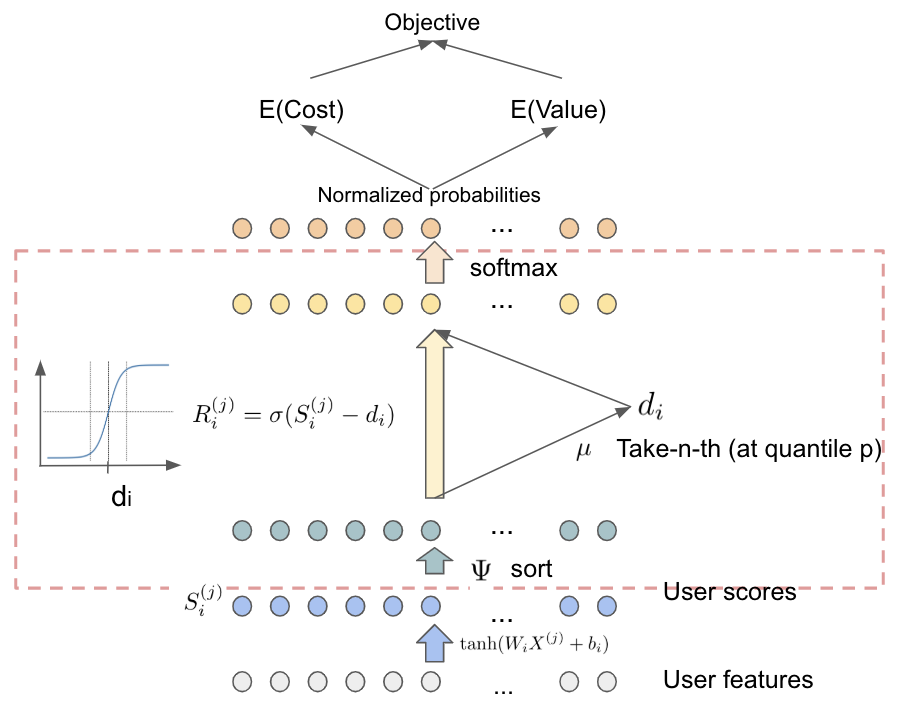
\includegraphics[width=\linewidth]{figures/fqr_figure} 
%  \caption{Illustration of the Fixed-Quantile-Ranking algorithm.} 
%\end{figure} 

\subsection{Sequential Causal Ranking Model} 
We now consider the cadence of treatments. For instance, when a user was treated in last period, her reaction to treatment in current period may be different. Or when users are treated too frequently, negative effects may accumulate. In this section, we describe a causal learning algorithm to capture short-term and long-term correlations across time. We perform causal learning with the ranking function $f$ which works with temporal sequences. Concretely, we apply recurrent neural networks to model temporal states of users. The input to this system is a feature vector for a user at any given time period. This feature vector contains information with common characterizations of the user in that period. 

\begin{figure}[h]
\label{seq_fig1}
  \centering
  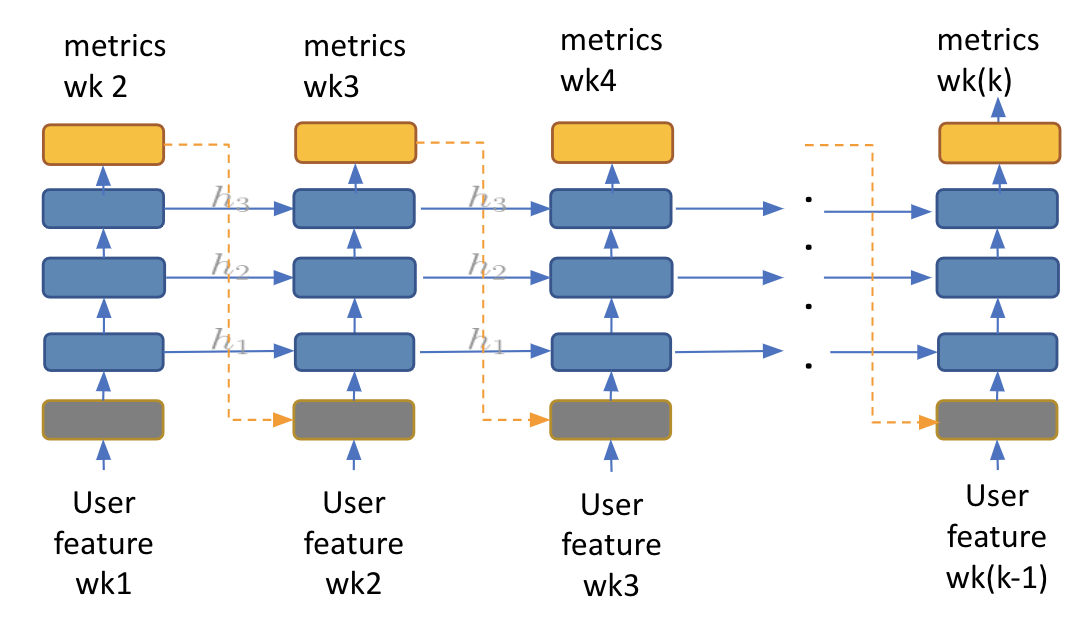
\includegraphics[width=0.75\linewidth]{figures/seq_fig1}
  \caption{Sequential representation of user states.}
  \vspace{-0.1cm}
\end{figure} 
\vspace{-0.1cm}
To construct an architecture that systematically correlates the sequence of states, and take into account the recurrent treatment labels, we resort to deep learning methods. First, the optimization objective in the previous section is abstracted into an epitomic module illustrated in Figure~\ref{fig:crll_module} which we call the \emph{Causal Ranking Loss Layer (CRLL)}. In this illustration, the operations to obtain ranking scores, separate cohorts, normalize and compute eventual objective is summarized into one module which takes in treatment assignment and other metric labels, as well as ranking model score. 
\vspace{-0.2cm}
\begin{figure}[h]
  \centering
  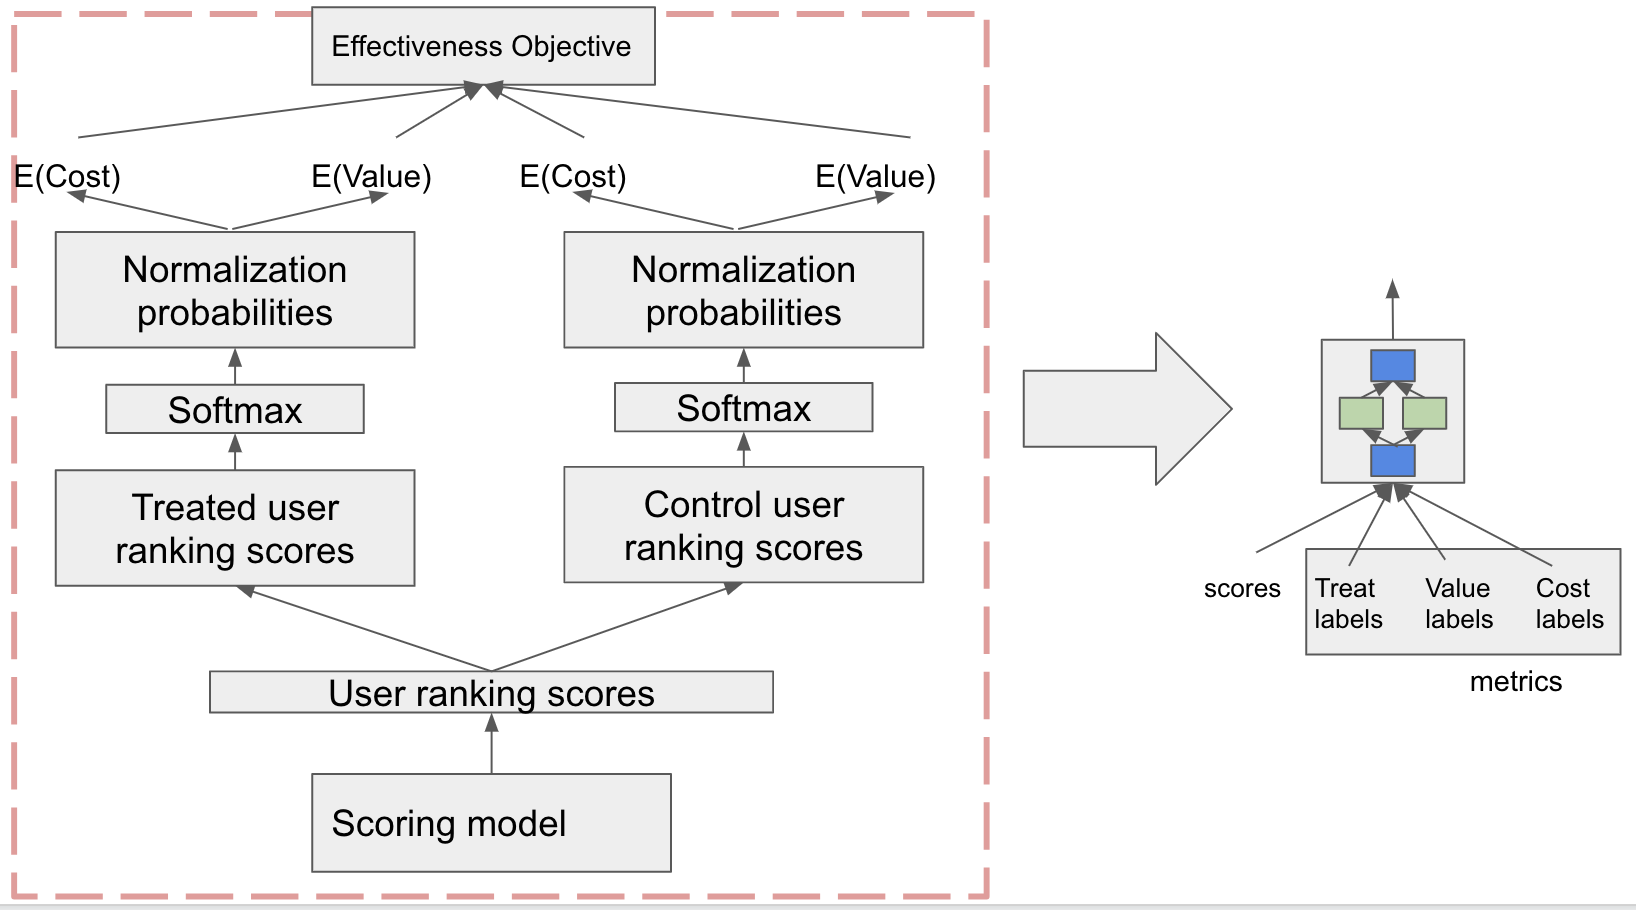
\includegraphics[width=\linewidth]{figures/crll_module}
  \caption{Causal Ranking Loss Layer.}
  \label{fig:crll_module}
\end{figure} 

\vspace{-0.2cm}
Next, we combine this module with recurrent networks to obtain a deep learning architecture which models the changes in user states across multiple stacked layers, and correlates with the experimental metrics. Concretely, instead of being a simple regressor, the ranker is now a recurrent network with recurrent connections across time. This allows states in the past to influence the future, while able to score users at any given time step. Also, the optimization objective is computed and measured at each time step. During optimization, we are able to combine the errors from objective at all time-steps to optimize the recurrent ranker.  

In this recurrent model, we not only consider the user inputs at this time step, but also the metric outputs of the previous time step, this is analogous to the architecture of sequence to sequence models~\cite{sutskever2014sequence}~\cite{wu16google}. 

\begin{figure}[h] 
\label{seq_fig2} 
  \centering 
  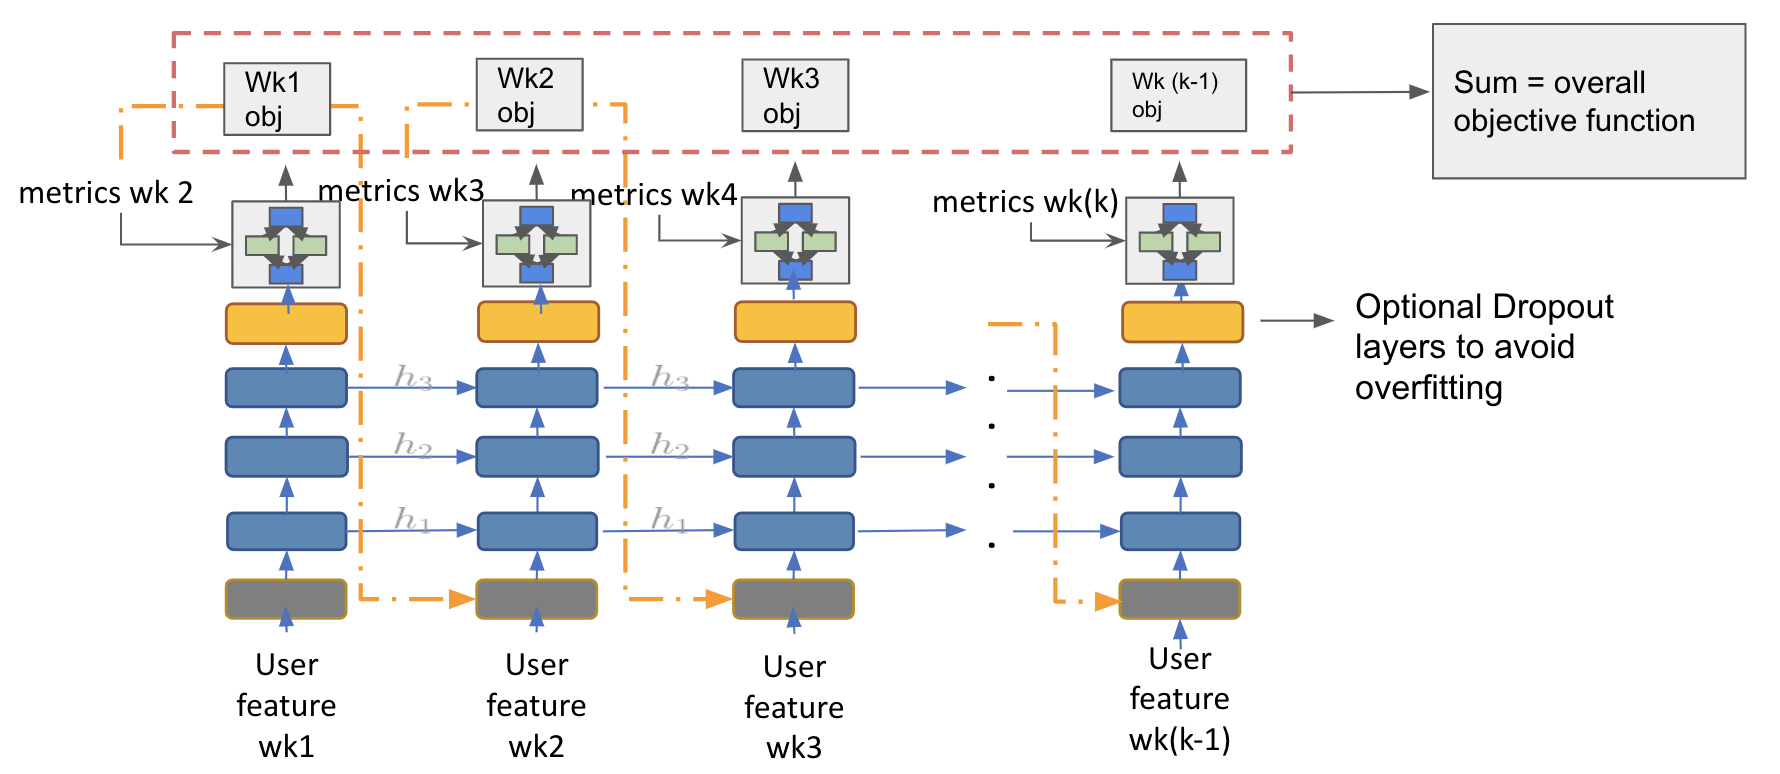
\includegraphics[width=\linewidth]{figures/seq_fig2} 
  \caption{Optimization objective function modularized to take in metrics and sampler/ranker score.} 
\end{figure} 

\subsection{Evaluation Methodology} 
The business objective is to achieve most incremental user retention with a given  cost budget. The retention and cost here are two critical values to trade-off. 

\textbf{\emph{Cost Curve}}. With two treatment outcome $\tau^{r}$ and $\tau^{c}$, we draw a curve and use cost as X-axis and retention as Y-axis as the illustration below. 
\vspace{-0.1cm}
\begin{figure}[h] 
\label{cost_curve_illustration} 
  \centering 
  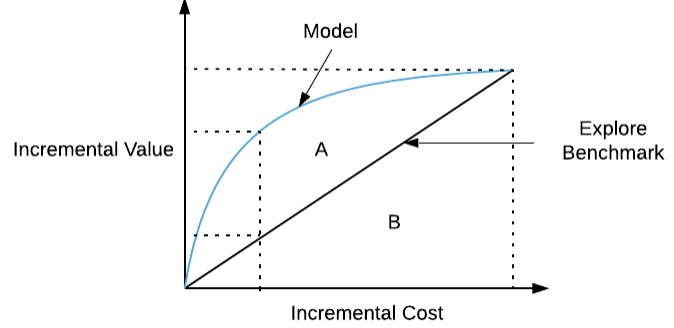
\includegraphics[width=\linewidth]{figures/cost_curve_illustration} 
  \caption{Illustration of the Cost-Curve.} 
\end{figure} 
Samples are ordered by the effectiveness score $S_i = f(X_i)$ on the cost curve. For each point on the curve, we take the number of treatment samples at this point on the curve, multiplied by ATE (Average Treatment Effect) of this group. 
\begin{align*}
\#\{T_i = 1 | S_i > S_i^{pth}\} \times ATE(x_i | S_i > S_i^{pth})
\end{align*}
Therefore each point represents aggregated incremental cost and value, usually both increasing from left to right. From origin to right-most of the curve, points on the curve represents the outcome if we include $p\%$ of the population for treatment, $p\in[0, 100]$.
% Note we can score the samples for both treatment and control as $f$ doesn’t depend on $W$. Here the function $f$ is the one we mentioned in previous sections. 

%Returning to the cost curve, as you increase the percent $p$ of samples to be included for each point, the aggregated incremental cost and value would increase (since you include more samples and assume treatment effect is non-negative). So the end point of the cost curve (top right) is the one that includes all samples. And the origin (down left) is the one includes no sample. 

If the score $S_i$ is randomly generated, the cost curve should be a straight line. If the score is generated by a good model, then the curve should be above the benchmark line, meaning for the same level of incremental cost, samples are selected to achieve higher incremental value. 

\textbf{\emph{Area Under Cost Curve (AUCC)}}. Similar to Area Under Curve of ROC curve, we define the normalized area under cost curve as  the area under curve divided by the area of rectangle extended by maximum incremental value and cost, or the area ratio $\frac{A + B}{2B}$. A and B are the area shown in the cost curve figure. So the AUCC value should be bounded within [0.5, 1) and larger the AUCC, generally better the model. 
%A is the area between model curve and the random benchmark line, and B is the area under random benchmark line. The equivalent formula for AUC of ROC curve is (A+B)/2B = A/2B + 0.5 where A/B is the value that matters. The theoretical upper bound of A is B (the symmetric upper triangle), which means with no incremental cost we can achieve all incremental value from the sample. 

\section{Empirical Results} 
\label{sec:empirical_results} 

In this section, we will cover the empirical results to compare proposed algorithms with prior art approaches (Causal Forest, R-Learner) on production data and pubic datasets. We will first describe the experiment data set and experiment setup in production. Then we would analyze both offline and online test results. In summary, cost curve offline evaluation is consistent with real-world online result and our proposed methods perform significantly better versus previous methods. 

\subsection{Experiments} 
The application goal of our model is to rank users from most effective to least effective, so that the overall market-wide metrics are optimized. As stated in algorithm section, we train our model on data logged from previous experiments with treatment assignment logs and the actual outcomes. 

\subsubsection{Experiment with Production Data} 
\label{sec:explore_exploit_exp} 
We adopt an explore and exploit experimental set-up in the paradigm of reinforcement learning~\cite{liu2018explore} and multi-armed bandits~\cite{katehakis1987multi}~\cite{li2010contextual}. We launch experiment algorithms in a cyclic fashion. For each cycle we have 2 experiments: explore and exploit, which contains non-overlapping sets of users. The explore experiment is randomly given, and serves to collect data from all possible scenarios. On the other hand, exploit applies model and other product features to optimizes performance. The experiment design is illustrated in the following chart.  
\begin{figure}[h] 
\label{explore_exploit_chart} 
  \centering 
  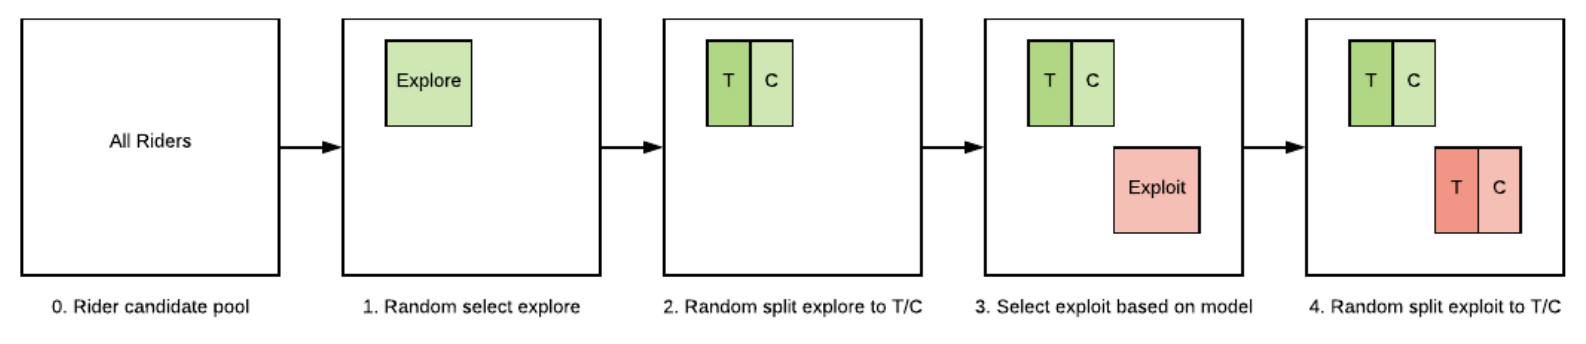
\includegraphics[width=\linewidth]{figures/explore_exploit_chart} 
  %\caption{.} 
\end{figure} 

\emph{Explore}. Users are randomly selected without any product specific algorithm, into explore experiments from the predefined user candidate pool. This allows us to collect an unbiased dataset which represents the whole population. Once users are selected, we then randomly give treatment / control assignment with a fixed probability\footnote{The number of samples in explore is solely determined by the budget.}. 

\emph{Exploit}. Excluding users already in explore experiments, based on model and budget we select users into exploit experiments. This exploit group is for product application. %Once users are selected, we then randomly give treatment / control assignment with a fixed probability. %When we have multiple exploits powered by different models, we will split the candidate pool into multiple (after excluding explore samples) subpool and launch exploit in each subpool. 

%Promotion product. We use Ride & Save type as our promotion structure. At the start of every cycle (cycle could be 1 or multiple weeks), user who received the promo will get notification (email, push and in-app messaging) telling them they get a promo and it’s valid through the whole cycle (with certain dollar cap and redemption frequency limit). 

%After the experiment period, we also have 4 blackout weeks that users who were censored during the experiment week will not get any other promotion during these blackout weeks. This helps us get the clean 4 week retention and cost outcome $Y^r$, $Y^c$.

We use explore for model training and offline performance evaluation and exploit for online performance evaluation. 
We collect data from experiments following this design. For each sample, we will log their feature constructed with data before experiment starts, experiment label (explore or exploit), treatment control assignment and outcomes (value and cost). Outcomes are aggregated within the experiment period. Value outcome could be any arbitrary desired business value the specific definition of which is unrelated to the algorithm, while cost outcome is also arbitrary undesired cost. %could be anything cost measures such as spend or negative net profit. 
%(the cycle while promo is valid)

\textbf{Production Data} To obtain data for model training and offline evaluation, we utilize a randomized \emph{explore} online experiment. We first randomly allocating users to control and treatment cohorts (A/B). For the treatment cohort, we give all users treatment.  In this experiment we collected millions of user level samples in multiple experiment periods. Following is an illustrative table for the dataset we collected. %We use real-time trip features, spatio-temporal features and user historical features for our modeling. 

\begin{table} 
  \caption{Example production dataset}
  \label{tab:example_data}
  \begin{tabular}{llllll}
    \toprule
    user id & strategy & $X_i$ & $T_i$& $Y^r$ & $Y^c$ \\
    \midrule
    A & explore & $(1.2, 3, ...)$ & $1$& $3$ & $2.3$ \\
    \midrule 
    B & exploit & $(2.4, 1, ...)$ & $0$& $1$ & $0.1$ \\ 
    \bottomrule
\end{tabular}
\end{table}

% \begin{figure}[h] 
% \label{feature_table} 
%   \centering 
%   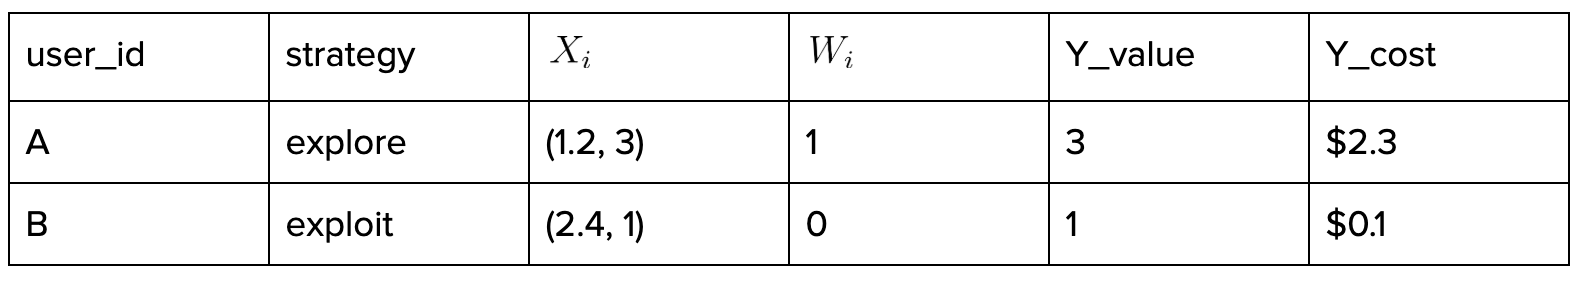
\includegraphics[width=\linewidth]{figures/feature_table} 
%   %\caption{.} 
% \end{figure} 

\textbf{Sequential Production Data} We extracted sequences of user features, treatment assignment, and outcomes as data from multiple cities. The data is extracted on a certain cadence for multiple cycles. This results in millions distinct users and multi-million records from web service logs. We split the data into training, validation and test with 50\%, 20\% and 30\%. %We combine treatment with small differences to increase the density of data across time and mitigate sequence sparsity. 

To deal with missing data per user across different cycles, we mask training and evaluation processes only with existent data. Only errors from objective function where sequential data exists is taken into account during model learning. For evaluation, the metrics are computed without missing data. When data is missing at any time step, we use a zero user feature vector as input to the model. This removes any influence to the recurrent computation of the LSTM's. 
\vspace{-0.3cm}
\subsubsection{Causal Experiments Designed with Public Datasets} 

The effectiveness of our proposed causal models is mainly experimented with production data. To ensure reproducibility we also experiment on public datasets. We make assumptions to select treatment assignment and outcomes on available data vectors to design simulated experiments for our proposed causal models. 

\textbf{US Census 1990} The US Census (1990) Dataset (Asuncion \& Newman, 2007~\cite{uscensulink} contains data for people in the census. Each sample contains a number of personal features (native language, education...). The features are pre-screened for confounding variables, we left out dimensions such as other types of income, marital status, age and ancestry. This reduces features to d = 46 dimensions. Before constructing experiment data, we first filter with several constraints. We select people with one or more children (\emph{`iFertil'} $\leq$ 2), born in the U.S. (\emph{`iCitizen'} = 0) and less than 50 years old (\emph{`dAge'} $<$ 5), resulting in a dataset with $225814$ samples. We select `treatment' label as whether the person works more hours than the median of everyone else, and select the income (\emph{`dIncome1'}) as the gain dimension of outcome for $\tau_r$, then the number of children (`iFertil') multiplied by $-1.0$ as the cost dimension for estimating $\tau_c$. The hypothetical meaning of this experiment is to measure the cost effectiveness, and evaluate who in the dataset is effective to work more hours. 
%\footnote{Full list of features are given in the Supplementary Materials}. 

\textbf{Covertype Data} The Covertype Dataset (Asuncion \& Newman, 2007) contains the cover type of northern Colorado forest areas with tree classes,  distance to hydrology, distance to wild fire ignition points, elevation, slope, aspect, and soil type. We pre-filter and only consider two types of forests: \emph{`Spruce-Fir'} and \emph{`Lodgepole Pine '}, and use data for all forests above the median elevation. This results in a total of $247424$ samples. After processing and screening for confounding variables, we use 51 features for model input. With the filtered data, we build experiment data by assuming we are able to re-direct and create water source in certain forests to fight wild fires, but also like to ensure the covertype trees are not imbalanced by changing the hydrology with preference to `Spruce-Fir'. Thus, the treatment label is selected as whether the forest is close to hydrology, concretely, distance to hydrology is below median of the filtered data. The gain outcome is a binary variable for whether distance to wild fire points is smaller than median, and cost outcome is the indicator for `Lodgepole Pine' (1.0, undesired) as opposed to `Spruce-Fir' (0.0, desired). 

Production data, public US Census and Covtype datasets are split into 3 parts: train, validation and test sets with respective percentages 60\%, 20\%, 20\%. We use train and validation sets to perform hyper-parameter selection for each model type. The model is then evaluated on the test set. 

\subsubsection{Model implementation details} In this section we briefly give the implementation details of our models. 

\emph{\textbf{Quasi-oracle estimation (R-Learner)}}. We use Linear Regression\footnote{Using SKLearn library's Ridge Regression with 0.0 as the regularization weight.} as the base estimator. Since the experiment cohorts are randomly selected, we use constant treatment percentage as propensity in the algorithm. Since we need to define one CATE function for R-learner, we use the R-learner to model the gain value incrementality with $\tau_r$. 

\emph{\textbf{Causal Forest}}. We leverage the generalized random forest (\emph{grf}) library in R~\cite{wager2018estimation}~\cite{grflink}. For details, we apply causal forest with 100 trees, 0.2 as alpha, 3 as the minimum node size, and 0.5 as the sample fraction. We apply the ratio of two average treatment effect functions in ranking by training two causal forests. To rank users or other cardinalities with respect to cost vs gain effectiveness, we estimate the conditional treatment effect function both for gain ($\tau_r$) and cost ($\tau_c$), i.e. train two Causal Forest models. For evaluation, we compute the ranking score according to the ratio of the two $\frac{\tau_r}{\tau_c}$. 
For hyper-parameters, we perform search on deciles for parameters \emph{num\_trees}, \emph{min.node.size}, and at 0.05 intervals for \emph{alpha}, \emph{sample.fraction} parameters. We also leverage the \emph{tune.parameters} option for the \emph{grf} package, eventually, we found best parameters through best performance on validation set\footnote{Best parameters are the same for all three datasets we experimented: \emph{num\_trees}$=100$ (50 trees for each of the two CATE function, $\tau_r$, $\tau_c$), \emph{alpha}$=0.2$, \emph{min.node.size}$=3$, \emph{sample.fraction}$=0.5$}. 

\emph{\textbf{Duality R-learner}}. Similar to R-learner, we use Ridge Regression as the base estimator and constant propensity, and apply the model stated in Eq.~\ref{eq:update_lambda} for ease of online deployment. The iterative process to solve $\lambda$ in Eq.~\ref{eq:lagrangian_score} is inefficient as the value function $g$ here is piece-wise linear w.r.t $\lambda$. Since Ridge Regression is lightweight to train, in practice, we take the approach to select $\lambda$ with best performance on the validation set.\footnote{We determine the value of $\lambda$ through hyper-parameter search on deciles and mid-deciles, e.g. $\lambda\in \{0.001, 0.005, 0.01, 0.05\}; best $\lambda$ for production data is $0.1$, for US Census and Covertype data is $0.05$.} 

\emph{\textbf{Direct Ranking}}. We implement our deep learning based models with Tensorflow. To align with baseline and other methods in our experiments, we use a one layer with linear parameterization $\tanh(\mathbf{w}^T \mathbf{x} + b)$ as the scoring function, without weight regularization, the objective functions stated in the algorithm section are used. We use the Adam optimizer with learning rate 0.01 and default beta values. We compute gradients for entire batch of data, and run for 600 iterations. 

\emph{\textbf{Constrained Ranking}}. We experiment with the \emph{Top Quantile} dynamic pooling operator. In addition to using a linear scoring function, we use a consistent quantile target at 40\%, and apply a starting sigmoid temperature of $0.5$, and use constraint annealing at increments of 0.1 every 100 steps of Adam optimizer. For constraint annealing, we validate and select different schedules. We note the dynamic quantile pooling offers a flexible lever $d^{(k)}$ to minimize objective function, making the optimization unstable. We stop the gradient on $d^{(k)}$ to disable the fast changing of this value. 

\emph{\textbf{Sequential Causal Ranking Model}}. We use Tensorflow framework (v2.0) and \emph{dynamic\_rnn} \emph{API} to implement recurrent neural networks. Specifically, we implement at multi-layer stacked LSTM as the recurrent ranking function. To speed-up training, we use minibatched algorithm for optimization. We simply take a larger minibatch, around 10,000 for gradients of sufficient quality, instead of complete dataset where each cohort have significant number of users. We optimize with Adam optimizer\footnote{Adam with learning rate of 0.01 and $\beta_1 = 0.5, \beta_2 = 0.995$.}. To avoid gradient explosion problems~\cite{sutskever2014sequence}, we train the model using $L2$ gradient clipping at threshold of $2.3$. 
\vspace{-0.2cm}
\subsection{Results on Causal Learning Models} 
Figure~\ref{production_data_result} shows the cost curve  for each model on production data test set. The baseline R-learner optimized for incremental gain $\tau_r$ could not account for the cost outcome and under-performs on our task. Thus we use Duality R-learner as a benchmark for all our experiments. Causal Forest also perform reasonably well. Direct Ranking out-performs previous models with \emph{10.7\%} improvement upon Duality R-learner, and Constrained Ranking algorithm is the best performing model on the production dataset, out-performing Duality R-learner by \emph{14\%}.
%\vspace{-0.2cm}
\begin{figure}[h] 
  %\centering 
  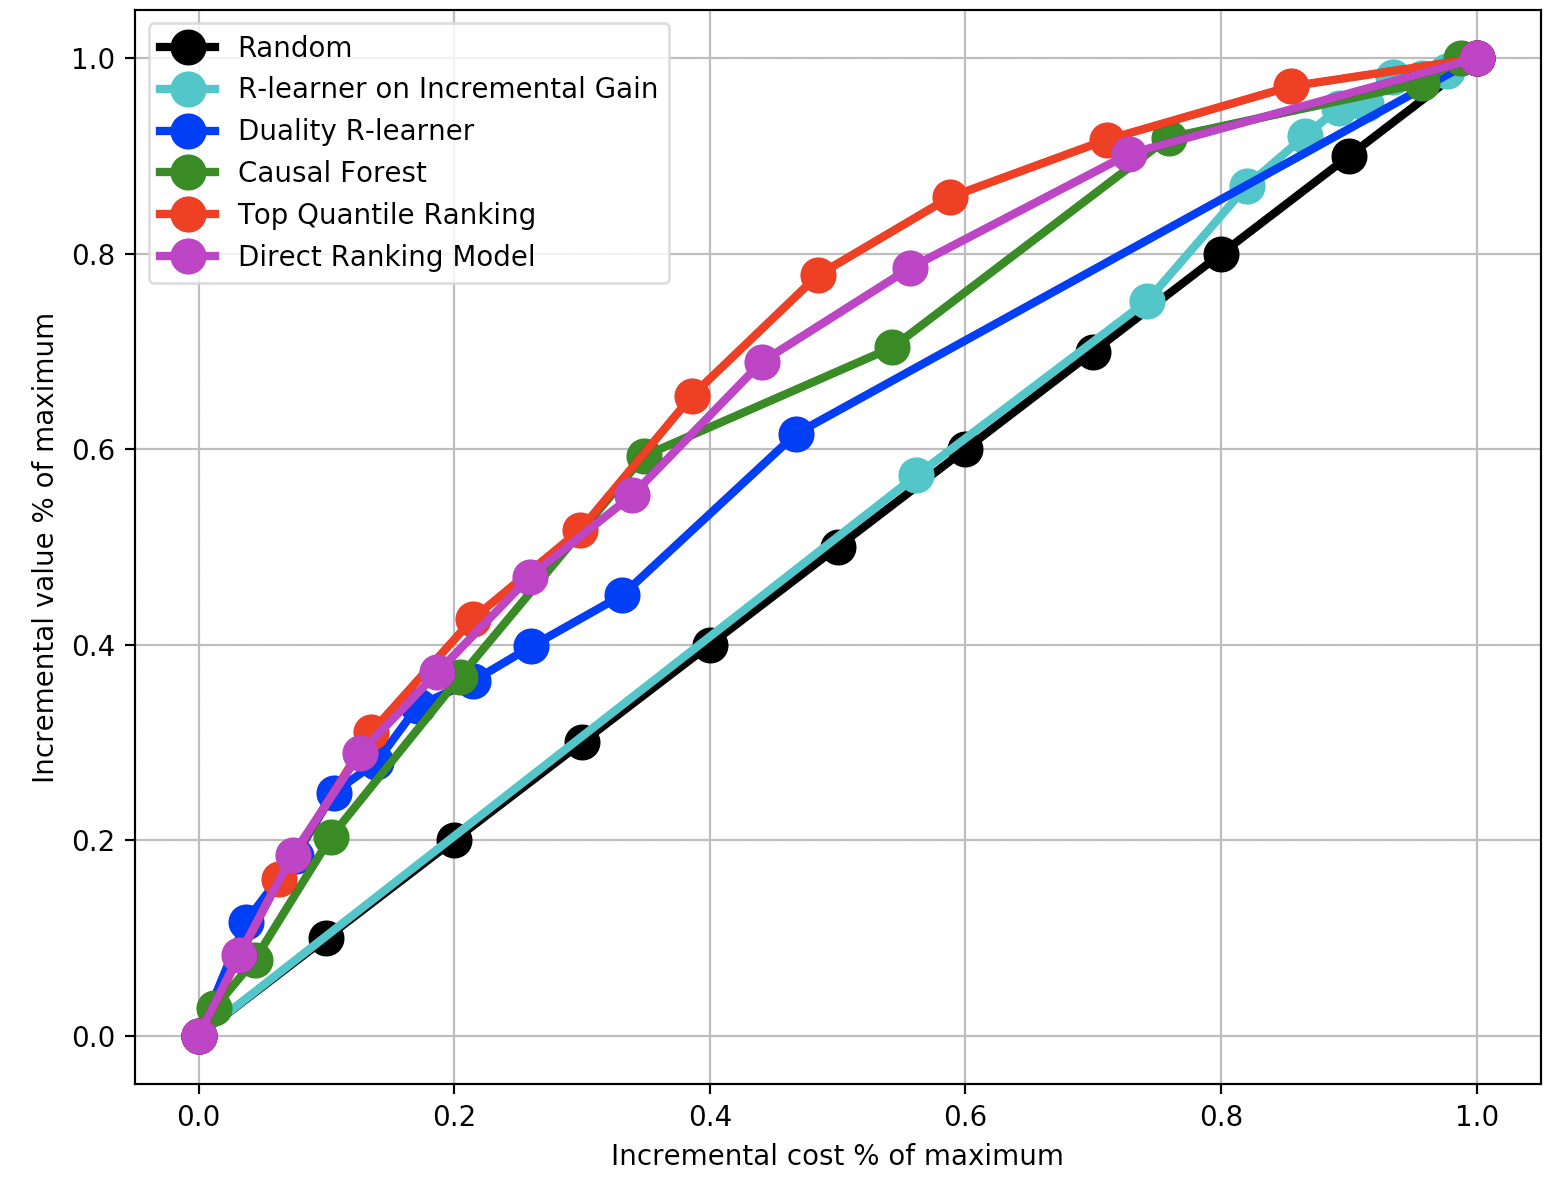
\includegraphics[width=0.75\linewidth]{figures/rxgy_result} 
  \caption{Cost-Curve results for Production data.} 
  \label{production_data_result} 
\end{figure} 
%\vspace{-0.4cm}
Figure~\ref{fig:uscensus_result} shows results of causal models on US Census. The baseline R-learner on gain performs slightly better due to less cost impact. Duality R-learner still works reasonably well. Direct Ranking and Constrained Ranking out-performs Duality R-learner by \emph{2.8\%} and \emph{21.2\%}, respectively to AUCC \emph{0.58} and \emph{0.69}. 
\begin{figure}[h] 
  %\centering 
  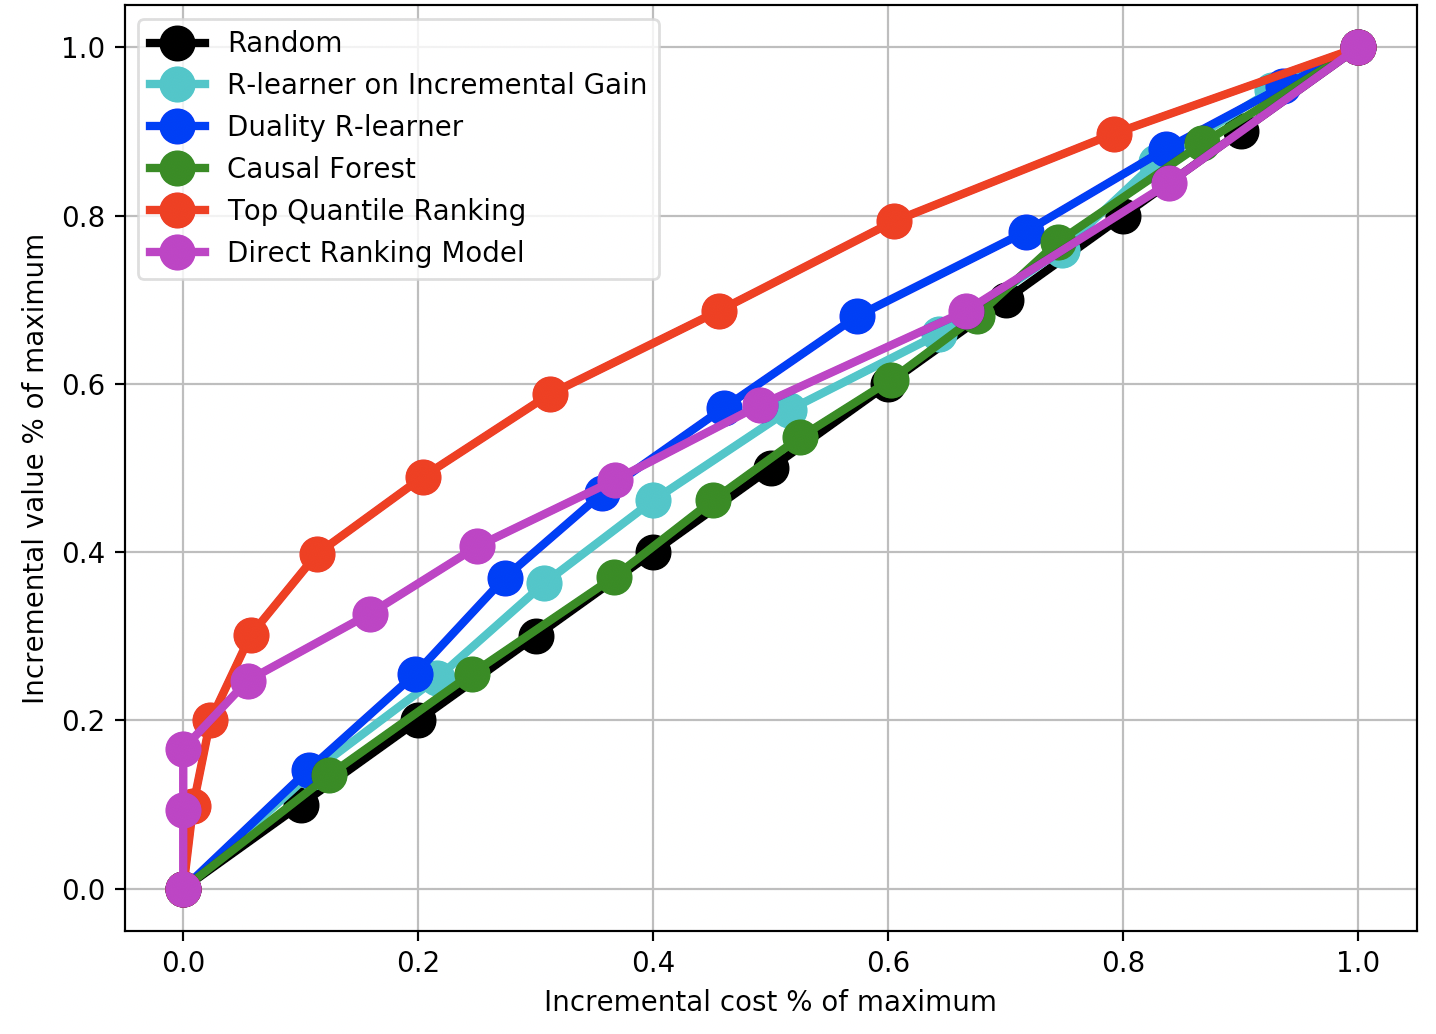
\includegraphics[width=0.75\linewidth]{figures/uscensus_result} 
  \caption{Cost-Curve results for public US Census data.} 
  \label{fig:uscensus_result} 
\end{figure} 
\vspace{-0.1cm}
Figure~\ref{fig:covtype_result} shows results of causal models on Covtype datasets. The optimization problem on this dataset is easier as results on multiple models are better. Direct Ranking and Constrained Ranking out-performs Duality R-learner by \emph{7.3\%} and \emph{17.9\%}, with AUCC for Constrained Ranking algorithm as high as \emph{0.92}. 

\begin{figure}[h] 
  %\centering 
  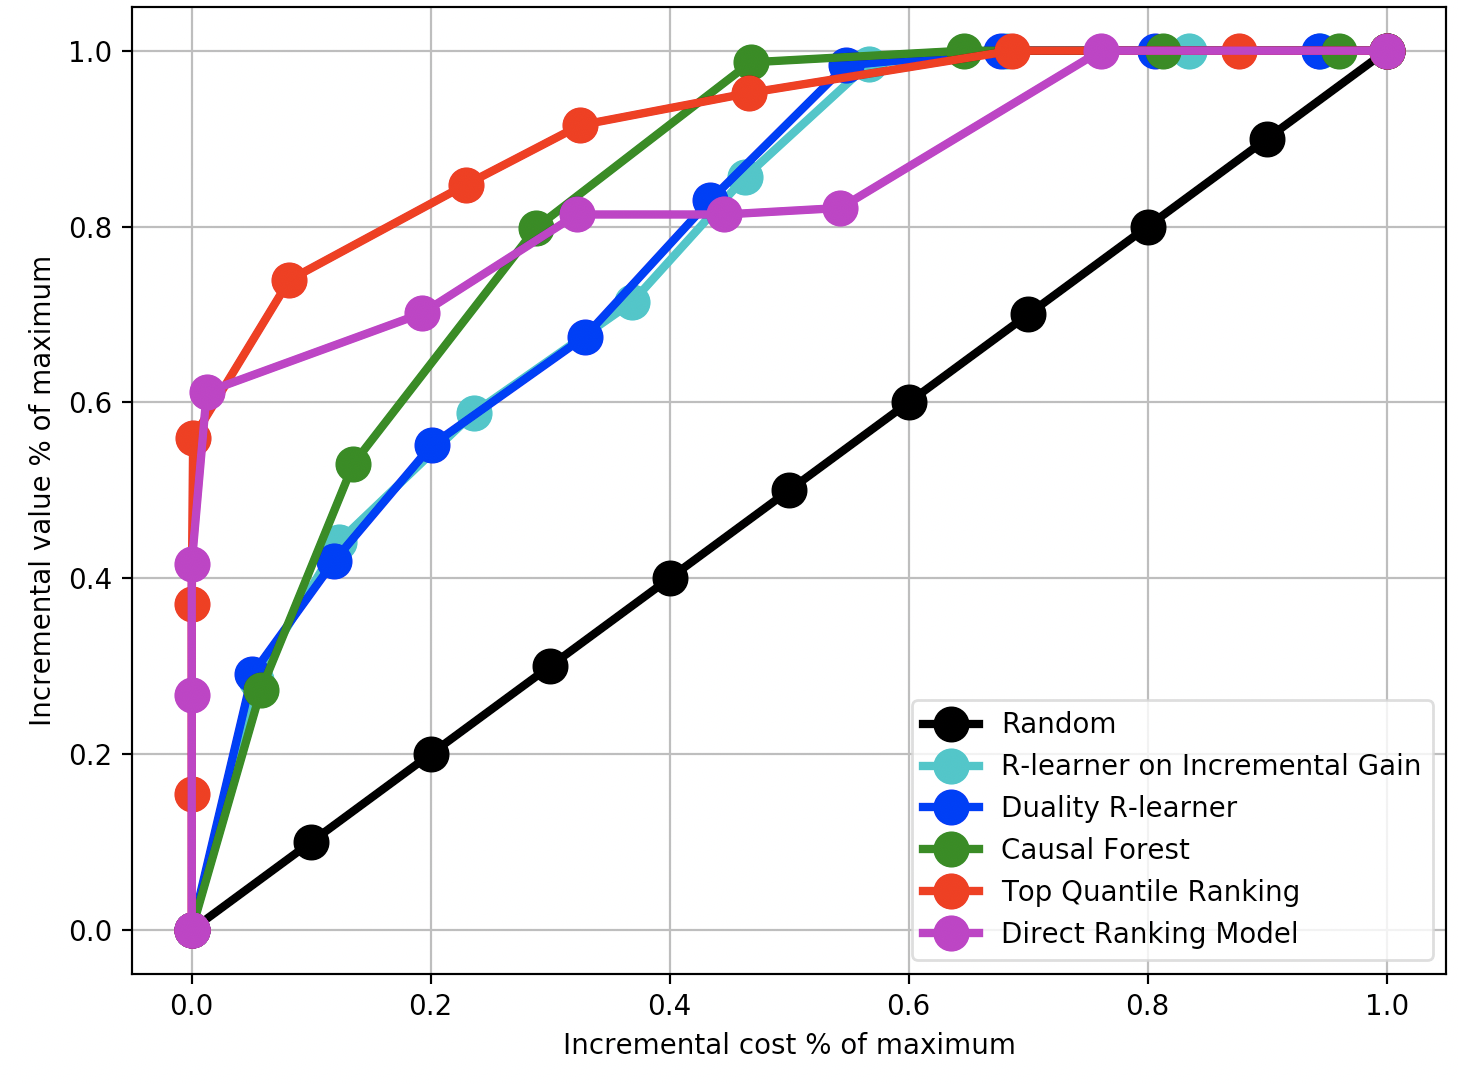
\includegraphics[width=0.75\linewidth]{figures/covtype_result} 
  \caption{Cost-Curve results for public Covtype data.} 
  \label{fig:covtype_result} 
\end{figure} 
Table~\ref{tab:summary_result_table} shows results Constrained Ranking and Direct Ranking algorithms are significantly better, more than \emph{25\%} in terms of AUCC, than R-learner on gain outcome, and out-performs Duality R-Learner by around \emph{10\%}. One example for cost effectiveness is to look at the vertical dash line at $20\%$ of total incremental cost, we can achieve 2X more incremental retention than random selection by using our causal models. This can result in 50\% reduction in cost. 
\begin{table}
  \caption{Summary of AUCC results across models and datasets.} 
  \label{tab:summary_result_table}
  \begin{tabular}{llllll}
    \toprule
    Algorithm & Prod. &\% imp. & USCensus &Covtype \\ 
    \midrule 
    Random & 0.500 && 0.500 & 0.500 \\
    \midrule 
    R-learner G & 0.514 && 0.533 & 0.779 \\
    Duality R-learner & 0.599 &0.0\%& 0.567 & 0.783 \\
    Causal Forest & 0.656 &9.5\%& 0.510 & 0.832 \\
    Direct Ranking & \textbf{0.663} &10.7\%& \textbf{0.583} & \textbf{0.840} \\
    Constrained Ranking & \textbf{0.685} &14.4\%& \textbf{0.687} & \textbf{0.915} \\
    \bottomrule
\end{tabular}
\end{table} 

The Direct Ranking Model has been deployed in production and operates in multiple regions all over the world. We present performance for DRM and Causal Forest in our online environment. Unlike the full cost-curve metrics for offline evaluation, in online case, we could only measure one specific point on the cost curve for each model. The slope of the straight line between that point and origin measures the general cost effectiveness. This slope is given as $R$ in Eq.\ref{eq:slope_r}. If both models have similar spend level (similar value on x-axis), this slope would sufficiently capture the performance. 

\vspace{-0.1cm}
\begin{equation}
  \label{eq:slope_r}
  R = \frac{ATE^r(x_i|selected)}{ATE^c(x_i|selected)}
\end{equation}
\vspace{-0.1cm}

As mentioned in Section~\ref{sec:explore_exploit_exp}, we have both explore and exploit in our online setup. In this case when we try to test 2 models for comparison between DRM and Causal Forest, we will have 1 explore (random selection) and 2 exploits (model based selection). Within selected users we then random split them into treatment and control. To make the numerical metric uniform, we use $R$ for explore as benchmark and derive Eq.~\ref{eq:ratio_r}, which represents the relative efficiency gain compared to the benchmark. 

\vspace{-0.1cm}
\begin{equation}
  \label{eq:ratio_r}
  \frac{R_{exploit}-R_{explore}}{R_{explore}}
\end{equation}
\vspace{-0.1cm}

\begin{table}
  \caption{Summary of efficiency gain online results.} 
  \label{tab:online_result_table}
  \begin{tabular}{llllll}
    \toprule
    City & DRM & Causal Forest \\ 
    \midrule 
    A & \textbf{75.3\%} & 60.2\% \\
    B & \textbf{61.5\%} & 54.3\% \\
    C & \textbf{101.2\%} & 80.4\% \\
    \bottomrule
\end{tabular}
\end{table} 

Table~\ref{tab:online_result_table} shows online test results for 3 arbitrary regions. They are consistent with the offline results that all models perform  significantly better than explore and DRM consistently out-performs Causal Forest.  %We haven't included online results for Duality R-learner as it's not in our production system. 

\textbf{Results of Sequential Causal Ranking Model} We evaluate the recurrent sequential model with a sequence of user states and treatments. Since we show DRM performing well on datasets, Sequential Causal Ranking method is compared directly with DRM. As shown in Table~\ref{tab:scrm_results}, the model is evaluated across multiple architectures, and we show the objective function value for training data set and test set. This objective is a direct measure of effectiveness on the dataset as an efficiency ratio of cost vs gain, the lower the better. The SCRM consistently out-performs Direct Ranking Model, e.g. by \emph{38\%} with 2 layer [16, 16] units on test set, and by \emph{28\%} with 1 layer LSTM. We also show in Figure~\ref{fig:scrm_costcurve} the cost curve for SCRM with respect to DRM without the sequential model architecture. This illustrate the incorporation of recurrent models on sequential user states can significantly boost the performance of causal models on production data. 
\begin{table} 
  \caption{Sequential Causal Ranking Model Objective as Effectiveness Ratios.}
  \label{tab:scrm_results}
  \begin{tabular}{lllll}
    \toprule
    Architecture&HSCL&. &Baseline& \\
    \midrule
    layers [num units] & Train & Test &Train & Test\\ 
    \midrule 
    1 layer LSTM $[6]$ & 7.17 & 7.80 & 8.01& 10.00 \\
    1 layer LSTM $[16]$ & 6.89 & 8.35 & 7.69& 8.93 \\
    2 layer LSTM $[16, 16]$ & 5.90 & \textbf{6.97} & 8.39& \textbf{9.65} \\
    3 layer LSTM $[8, 8, 8]$ & 7.35 & 8.64 & 7.97 & 9.73 \\
    \bottomrule
\end{tabular}
\end{table}

\begin{figure}[h] 
  \centering 
  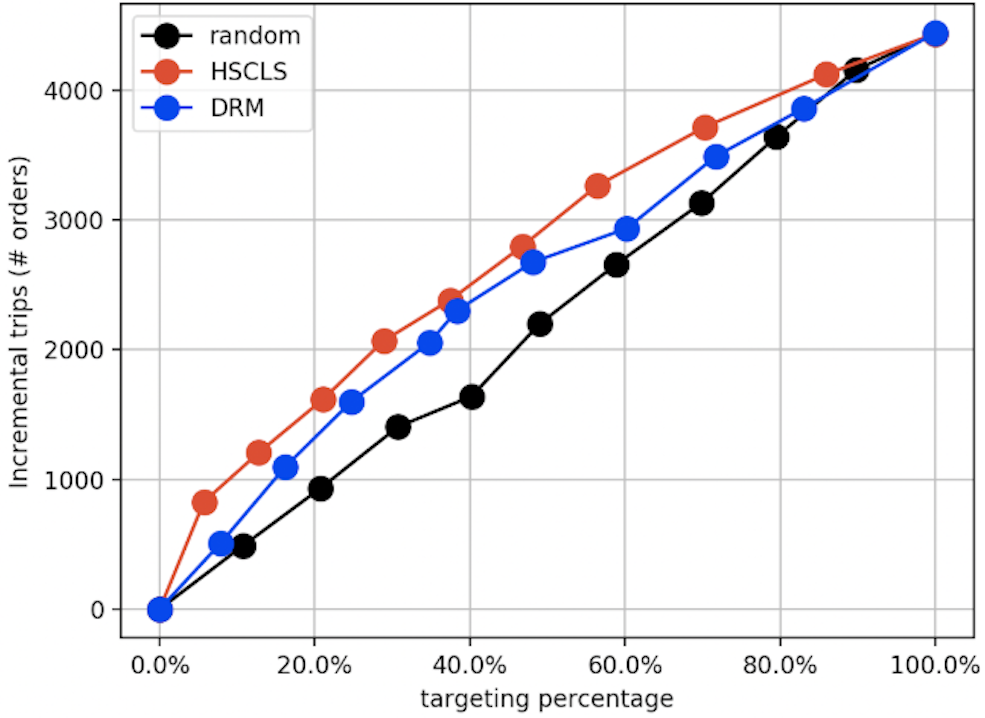
\includegraphics[width=0.75\linewidth]{figures/hscl_result} 
  \caption{Cost-curve results for sequential causal ranking model on held-out test set.} 
  \label{fig:scrm_costcurve} 
\end{figure} 

%\begin{figure}[h] 
%\label{drm_result_table} 
%  \centering 
%  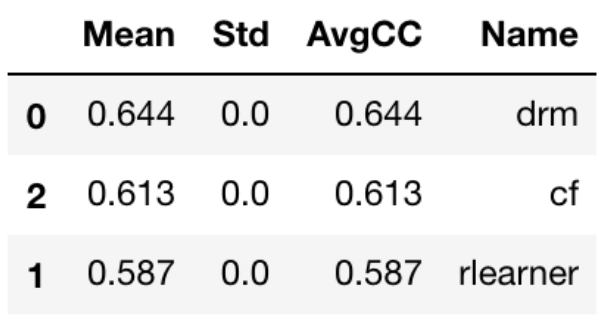
\includegraphics[width=0.4\linewidth]{figures/drm_result_table} 
%  \caption{Cost-Curve results for DRM vs rlearner vs causal forest %model.} 
%\end{figure} 

\section{Conclusion and Future Work} 

\subsection{Conclusion} 
We propose a novel ranking method to optimize heterogeneous treatment effect for user retention. The method combines prediction and optimization into one single stage and provides a loss layer that can be incorporated with any deep learning structure. We also provide an empirical evaluation metric and adjustments for existing estimator for the  treatment effect optimization problem. We evaluate various methods empirically both offline and online. Our proposed method achieves significantly better performance than explore benchmark and existing estimators. After successful test, this method has been deployed to production and is live in many regions all over the world.

\subsection{Future Work} 
\emph{Smart Explore/Exploit}. In current work we use epsilon-greedy explore, where we split a fixed percentage of budget to spend on fully randomized explore to collect data for model training. However, this will sacrifice the overall performance and is suboptimal. As a better approach, we will try to use multi-arm bandit or Bayesian optimization framework to guide our smart explore based on the model uncertainty. 

\emph{Deep Embedding}. Raw time and geo features are extremely sparse. Various embedding techniques have been used for sparse features but none of them is specifically for treatment effect. As treatment effect is different from its underlying outcome, the embedding should also be different. Now that we have a general loss layer which could be incorporated with any deep learning structure, we could start to work on the embeddings specifically for treatment effects. 

%From the table below we can observe a consistent improvement (the lower the better) with using the sequential causal learning system. 

%%
%% The next two lines define the bibliography style to be used, and
%% the bibliography file.
\bibliographystyle{ACM-Reference-Format}
\bibliography{references}

\end{document} 

%\endinput 
%% 
%% End of file `sample-authordraft.tex'. 
